\chapter{Theory of Laser Coupled with Passive Cavity}
\label{ch:Theory}
Semiconductor lasers with external cavities exhibit a variety of dynamical phenomena, depending on key parameters, comprising feedback strength, feedback delay, pump current, feedback type, and laser nonlinearity \cite{soriano2013complex}. Among all of them, the feedback sensitivity of laser diodes is governed essentially by the feedback parameters $C$, $X$ and $\kappa_{ext}$. In order to correctly consider the feedback effect in our tunable DBR laser, a three-mirror laser model and its equivalent two-mirror Fabry-Perot cavity are considered in \autoref{fig:laser_cavity_model}.
% The transmission coefficent across the interface, $t_2$, includes any scattering or coupling loss, so $r_2^2+t_2^2\neq1$, in general.

\begin{figure}[ht]
    \centering
    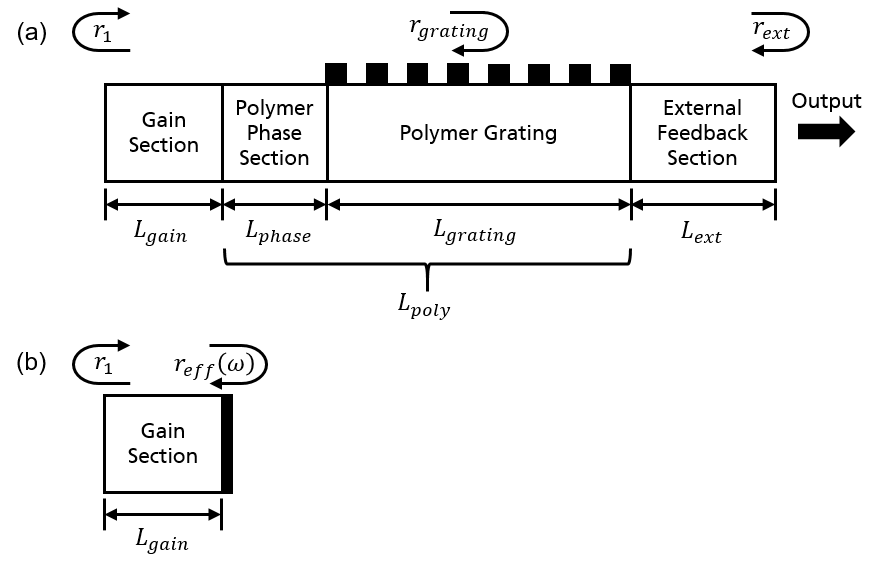
\includegraphics[width=.9\linewidth]{figures/laser_cavity_model.png}
    \caption{(a) DBR laser with external cavity and (b) its equivalent cavity with effective mirror to model the feedback effect. The InP gain section that possesses a length of $L_{gain}$ is equipped with a high reflection (HR) front facet and is but-coupled to the Polyboard. The Polyboard consists a phase and a grating section with a total length of $L_{poly}$ and the external cavity with a length of $L_{ext}$ after the grating section. $r_1$, $r_{grating}$ and $r_{ext}$ are amplitude reflectivities of the gain chip front facet, grating and external reflector respectively.}
    \label{fig:laser_cavity_model}
\end{figure}

The feedback coefficient, $C$, characterizes the level of feedback in relation to how it affects the mode structure of the laser, is defined as
\begin{equation}
    C=X\sqrt{1+\alpha^2}
\end{equation}
with
\begin{equation}
    X=\frac{\tau_{ext}}{\tau_{gain}+\tau_{poly}}\kappa_{ext}
\end{equation}
\begin{equation}
    \kappa_{ext}=\frac{r_{ext}}{r_{grating}}\qty(1-\abs{r_{grating}}^2)
\end{equation}
where $\tau=2nL/c$ is the roud trip time in the corresponding section, $\kappa_{ext}$ is the coupling coefficient from the grating reflector to the external cavity and $\alpha$ is the linewidth enhancement factor. Note that here the grating reflectivity $r_{grating}$ is considered as a static value, which leads to effective grating length $L_{eff}=tanh(\kappa L)/2\kappa$ shorter than the real grating length $L$ \cite{kuznetsov1988theory}. The $L_{eff}$ is then contained in the normal cavity and the rest of the grating is included in the external cavity.

The $C$ parameter indicates that the laser stability under feedback is affected both by external reflector $r_{ext}$ and external round-time delay $\tau_{ext}$. When $C<1$, usually for weak feedback and relatively short external cavities, the laser operates in a single mode lasing region and is phase dependent to the external feedback, when $C>1$, over one stable mode will appear and the laser will undergo a route-to-chaos behavior until it reaches coherence-collapse \cite{lenstra1985coherence} region, which is the region IV for the experimentally identified five distinct regimes of laser performance under feedback \cite{tkach1986regimes}. After the coherence-collapse region, if the feedback strength is even higher, the laser will operates in stable single mode again lasing with the compound cavity mode.

% Rate equation models of the field and phase including the time delay of the feedback field reveal unstable solutions and chaotic behavior at these high feedback levels \cite{tkach1986regimes}. The collapse begins at the transition to regime IV, where the normally small satellite peaks created by noise-induced relaxation oscillations (depicted in Fig. 5.23) grow larger and larger, eventually becoming comparable to the central peak and broadening the linewidth dramatically \cite{coldren2012diode}.

It is useful to identify the static lasing behavior by using the $C$ parameter, but in order to quantitatively model the laser under feedback, the equivalent two-mirror cavity by replacing the external feedback part with an effective mirror of reflectivity $r_{eff}(\omega)$ is considered
\begin{equation}
    r_{eff}(\omega)=r(\omega)e^{-i\varphi(\omega)}=\frac{r_{grating}(\omega)+r_{ext}W}{1+r_{grating}(\omega)r_{ext}W}
    \label{eq:effective_reflectivity}
\end{equation}
\begin{equation}
    W=e^{-2\alpha_{poly}L_{ext}}e^{-2i\beta_{poly}L_{ext}}
\end{equation}
where $\alpha_{poly}$ and $\beta_{poly}$ are the propagation loss and the propagation constant of the external cavity respectively, $r_{grating}(\omega)$ is the frequency-dependent complex amplitude reflectance of the grating reflector \cite{yariv1977periodic}.

The resonance equation $G$ for the effective laser cavity model is then given by \cite{vallone2011enhanced}
\begin{equation}
    G=r_1e^{-2i\tilde{\beta}_{gain}L_{gain}}r_{eff}(\omega)=\abs{G}e^{i\varphi(\omega)}
    \label{eq:RTG_RTP}
\end{equation}
with
\begin{equation}
    \tilde{\beta}_{gain}=\beta+i\beta_{i}=\beta+\frac{i}{2}(g-\alpha_{in})
    \label{eq:beta_gain}
\end{equation}
where the real part $\beta=2\pi n_{gain}/\lambda$ is the propagration constant inside the gain section, and the imaginary part consists of the modal gain $g$ and the internal loss $\alpha_{in}$ in the gain medium \cite{coldren2012diode}. Cavity modes are obtianed from \autoref{eq:RTG_RTP} for integer values of $\varphi/2\pi$; for the lasing mode $m$ at threshold we get
\begin{equation}
    \abs{G(\lambda_m)}=G_m=1,\ \varphi_m=2m\pi
    \label{eq:lasing_condition}
\end{equation}
these two conditions allow to numerically find the lasing mode wavelength $\lambda_m$.

% In 1980, Lang and Kobayashi published a rate equation model (the LK model) for a single-mode laser, describing the time evolution of the complex optical field and the carriers. They included the influence of the optical feedback by considering the interference of the laser field with its own coherent delayed field that had propagated once through the external cavity (Lang and Kobayashi, 1980). The model can be written as equations for the excess number of carriers $n(t)=N(t)-N_{th}$ with respect to the solitary threshold level $N_{th}$, and for the slowly varying complex electrical field amplitude $E(t)$:
% \begin{equation}
%     \dv{E(t)}{t}=\frac{1}{2}\qty(1+i\alpha)\xi n(t)E(t)+\kappa E\qty(t-\tau_f)e^{-i\omega_0\tau_f}
%     \label{Lang_Kobayashi_1}
% \end{equation}
% \begin{equation}
%     \dv{n(t)}{t}=\qty(p-1)\frac{I_{th}}{e}-\gamma_e n(t)-\qty[\Gamma_0+\xi n(t)]P(t)
%     \label{Lang_Kobayashi_2}
% \end{equation}

% The optical feedback is taken into account via the feedback term at the end of \autoref{Lang_Kobayashi_1}, including $\kappa$ as the feedback rate and $\tau_f$ as the delay time. The optical field is normalized such that $P(t)=\abs{E(t)}^2$ is the photon number, $\omega_0$ represents the angular optical frequency of the solitary laser, $\xi$ is the differential gain, $\Gamma_0=1/T_p$ is the cavity decay rate, and $\gamma_e=1/T_e$ is the inverse carrier lifetime. The bias current at the solitary laser threshold is denoted as $I_{th}$, $e$ is the electron charge, $p$ is the pump parameter, and $\alpha$ is the so-called linewidth enhancement factor discussed in more detail below. The excess phase $\phi_f$ that the opitcal field accmulates within theexternal cavity can be defined as $\phi_f=\omega_0\tau_f\mod2\pi$.

\section{Linewidth and Chirp Reduction}\label{sec:linewidth_and_chirp_reduction}
Linewidth and chirp reduction due to the optical feedback is related to the factor $F$, which is defined as \cite{kazarinov1987relation}
\begin{equation}
    F=1+A+B
    % F=1+\frac{1}{\tau_{gain}}\dv{\phi_{r_{eff}}}{\omega}+\frac{\alpha}{\tau_{gain}}\dv{\ln{r_{eff}}}{\omega}=1+A+B
    \label{eq:F_factor}
\end{equation}
with
\begin{equation}
    A=\frac{1}{\tau_{gain}}\dv{\varphi_{r_{eff}}}{\omega}
    \label{eq:F_factor_A}
\end{equation}
\begin{equation}
    B=\frac{\alpha}{\tau_{gain}}\dv{\ln{r_{eff}}}{\omega}
    \label{eq:F_factor_B}
\end{equation}
\begin{equation}
    \Delta\omega=\frac{\Delta\omega_0}{F}
    \label{eq:chirp_reduction}
\end{equation}
\begin{equation}
    \Delta\nu=\frac{\Delta\nu_0}{F^2}
    \label{eq:linewidth_reduction}
\end{equation}
where $\alpha$ is the linewidth enhancement factor, $\Delta\omega$, $\Delta\nu$ and $\Delta\omega_0$, $\Delta\nu_0$ are the chirp and linewidth with and without feedabck respectively. The parameter $A$ is the freqeuncy derivative of the $r_{eff}(\omega)$ phase in \autoref{eq:effective_reflectivity}, it denotes the ratio of the effecitve round trip time (cavity path length outside gain medium) to the round trip time in the gain section (gain section path length). It can be interperated as the ratio of the photon numbers outside to inside the gain medium, which remains nearly constant once the laser cavity is formed. By designing a cavity with a long external cavity, a large $A$ can be achieved. However, parameter $B$, representing the slope of the spectral reflectivity, is changed if the lasing mode is detuned. Additional reduction occurs only at the rising slope of the spectral peak of the external feedback which represents the contribution of the detuned loading effect and will be explained in \autoref{subsec:detuned_loading}.

% If $\Delta\omega_0$ is denoted as the adiabatic chirp in the absence of feedback, then the chirp with external cavity $\Delta\omega$ is obtained as \cite{kazarinov1987relation}
% \begin{equation}
%     \Delta\omega=\frac{\Delta\omega_0}{F}
%     \label{eq:chirp_reduction}
% \end{equation}
% if the spectral linewidth without external feedback is denoted by $\Delta\nu_0$, the spectral linewidth with the external cavity $\Delta\nu$ is simply obtianed as \cite{}
% \begin{equation}
%     \Delta\nu=\frac{\Delta\nu_0}{F^2}
%     \label{eq:linewidth_reduction}
% \end{equation}

Consider the five different feedback regions studied in \cite{tkach1986regimes}, the reduction factor at weak feedback ($C<1$) becomes \cite{coldren2012diode, petermann2012laser}
\begin{equation}
    F=1+C\cos(\phi_{ext}+\arctan\alpha)
    \label{eq:F_weak_feedback}
\end{equation}
where $\phi_{ext}=2\beta_{poly}L_{ext}$ is the round trip phase of the external cavity. \autoref{eq:F_weak_feedback} shows that at weak feedback, the linewidth can either be narrowed $\Delta\nu_0/(1+C)^2$ or broadened $\Delta\nu_0/(1-C)^2$ depending on the feedback phase. For strong feedback, which is more interesting and stable for the practical implementation, the factor $F$ becomes
\begin{equation}
    F=1+f_{ext}\frac{\tau_{ext}}{\tau_{gain}+\tau_{poly}}
    \label{eq:F_strong_feedback}
\end{equation}
with
\begin{equation}
    f_{ext}=\eta_{couple}R_{ext}
    \label{eq:F_f_ext}
\end{equation}
where $\eta_{couple}$ is the coupling coefficient between the normal cavity and external cavity. This parameter is included because for the design presented in \autoref{sec:design}, the feedback from the external cavity is not totally coupled back to the normal cavity. However, in this case $\eta_{couple}=1$.

With \autoref{eq:F_weak_feedback} and \autoref{eq:F_strong_feedback} we calculated the linewidth reduction factor $F^2$ versus the external cavity length as shown in \autoref{fig:F_reduction_factor}. $L_c$ indicates the length when the $C$ parameter goes over 1 and unstable laser behavior is expected. \autoref{fig:F_reduction_factor} is caculated under the assumption that the feedback comes from the chip edge, which is formed by a polymer/air interface and results in $R_{ext}=0.187$.

\begin{table}[ht]
    \centering
    \caption{Parameters used for linewidth reduction factor $F^2$ calculation.}
    \begin{tabular}{@{}lll@{}}
    \toprule
    Symbol        & Description                  & Value           \\ \midrule
    $L_{gain}$    & Active section length        & 300 $\mu m$     \\
    $L_{phase}$   & Phase section length         & 525 $\mu m$     \\
    $L_{grating}$ & Grating section length       & 699.84 $\mu m$  \\
    $L_{poly}$    & Polymer section length       & 1224.84 $\mu m$ \\
    $\alpha$      & Linewidth redcution factor   & -3              \\
    $R_{grating}$ & Grating reflectivity         & 0.3             \\
    $R_{ext}$     & External cavity reflectivity & 0.187           \\ \bottomrule
    \end{tabular}
    \label{tab:F_reduction_factor}
\end{table}

\begin{figure}[ht]
    \centering
    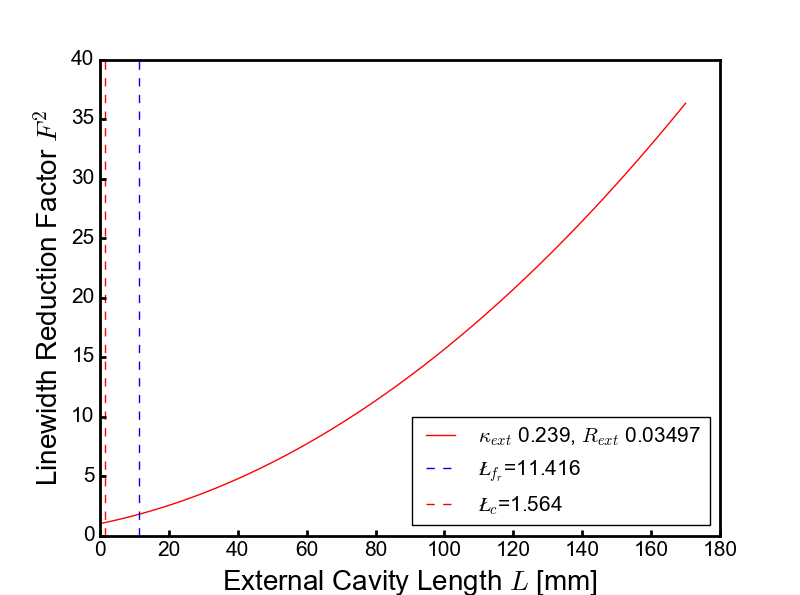
\includegraphics[width=.7\linewidth]{figures/F_reduction_factor.png}
    \caption{Calculated linewidth reduction factor $F^2$ assuming the feedback comes from the poly/air interface. Dashed vertical line $L_c$ indicates the length where the $C$ parameter exceeds 1 and unstable laser behavior is expected.}
    \label{fig:F_reduction_factor}
\end{figure}

\section{Bandwidth Enhancement}\label{sec:bandwidth_enhancement}
The maximum bit rate achieved by direct modulated lasers is limited by the well known resonance between carriers and photons \cite{coldren2012diode}. Many solutions have been proposed to overcome this restriction and three approaches to achieve broader bandwidth are explored in detail here. 
% (typically 1\textasciitilde{}10 GHz)
\subsection{Detuned Loading Condition}\label{subsec:detuned_loading}
The first mechanism identified to extend the modulation bandwidth of a semiconductor laser is the detuned loading effect which is due to the dispersion effect introduced by a coupled cavity \cite{vahala1984detuned, vahala1985observation} or by a distributed mirror (e.g. DBR \cite{feiste1998optimization, kjebon1997two, chacinski2010impact}). It can be achieved by positioning the lasing mode at a slightly higher wavelength respect to the minimum threshold gain condition, which means the lasing mode of a DBR laser is oscillating at the higher slope of its grating response. It is reported that when the laser is operating at the longer wavelength side, an enhancement of modulation speed, reduction of phase noise (linewidth), and suppression of FM modulation (chirping) can be achieved \cite{vahala1984detuned}. The detuned loading of the laser cavity increases the interaction between the photons and the free carriers in the laser cavity which will both increase the modulation bandwidth and reduce the variation of the carrier density during modulation \cite{kjebon2002experimental}. This is because, in the longer wavelength region, the increase in carrier density increases the material gain while reducing the mirror loss (i.e. increase the reflection from the grating). As a result, the effective differential gain is increased, which, in turn, reduces the effective linewidth enhancement factor \cite{vahala1984detuned, chacinski2010impact}.

\begin{figure}[ht]
    \centering
    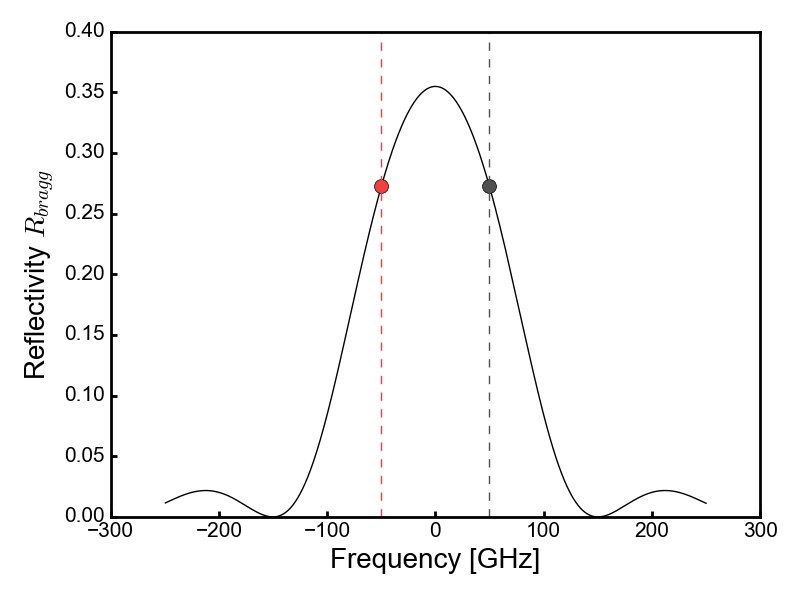
\includegraphics[width=.7\linewidth]{figures/detuned_loading_principle.png}
    \caption{Detuned loading condition with respect to the grating response. The red and grey dots correspond to the lasing mode detuend to the longer and shorter wavelength sides.}
    \label{fig:detuned_loading_principle}
\end{figure}


% \begin{figure}[!htb]
%   \begin{minipage}{0.48\textwidth}
%      \centering
%      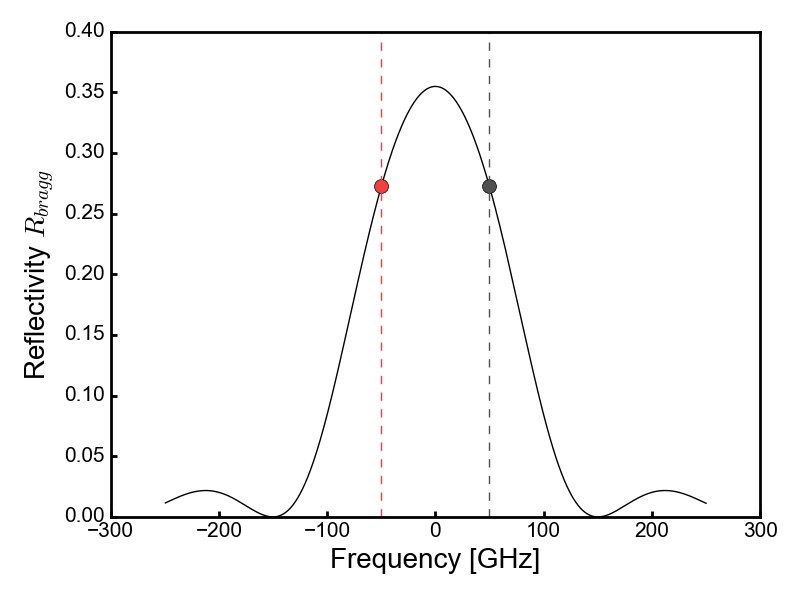
\includegraphics[width=.7\linewidth]{figures/detuned_loading_principle.png}
%      \caption{Detuned loading operation principle}
%      \label{fig:detuned_loading_principle}
%   \end{minipage}\hfill
%   \begin{minipage}{0.48\textwidth}
%      \centering
%      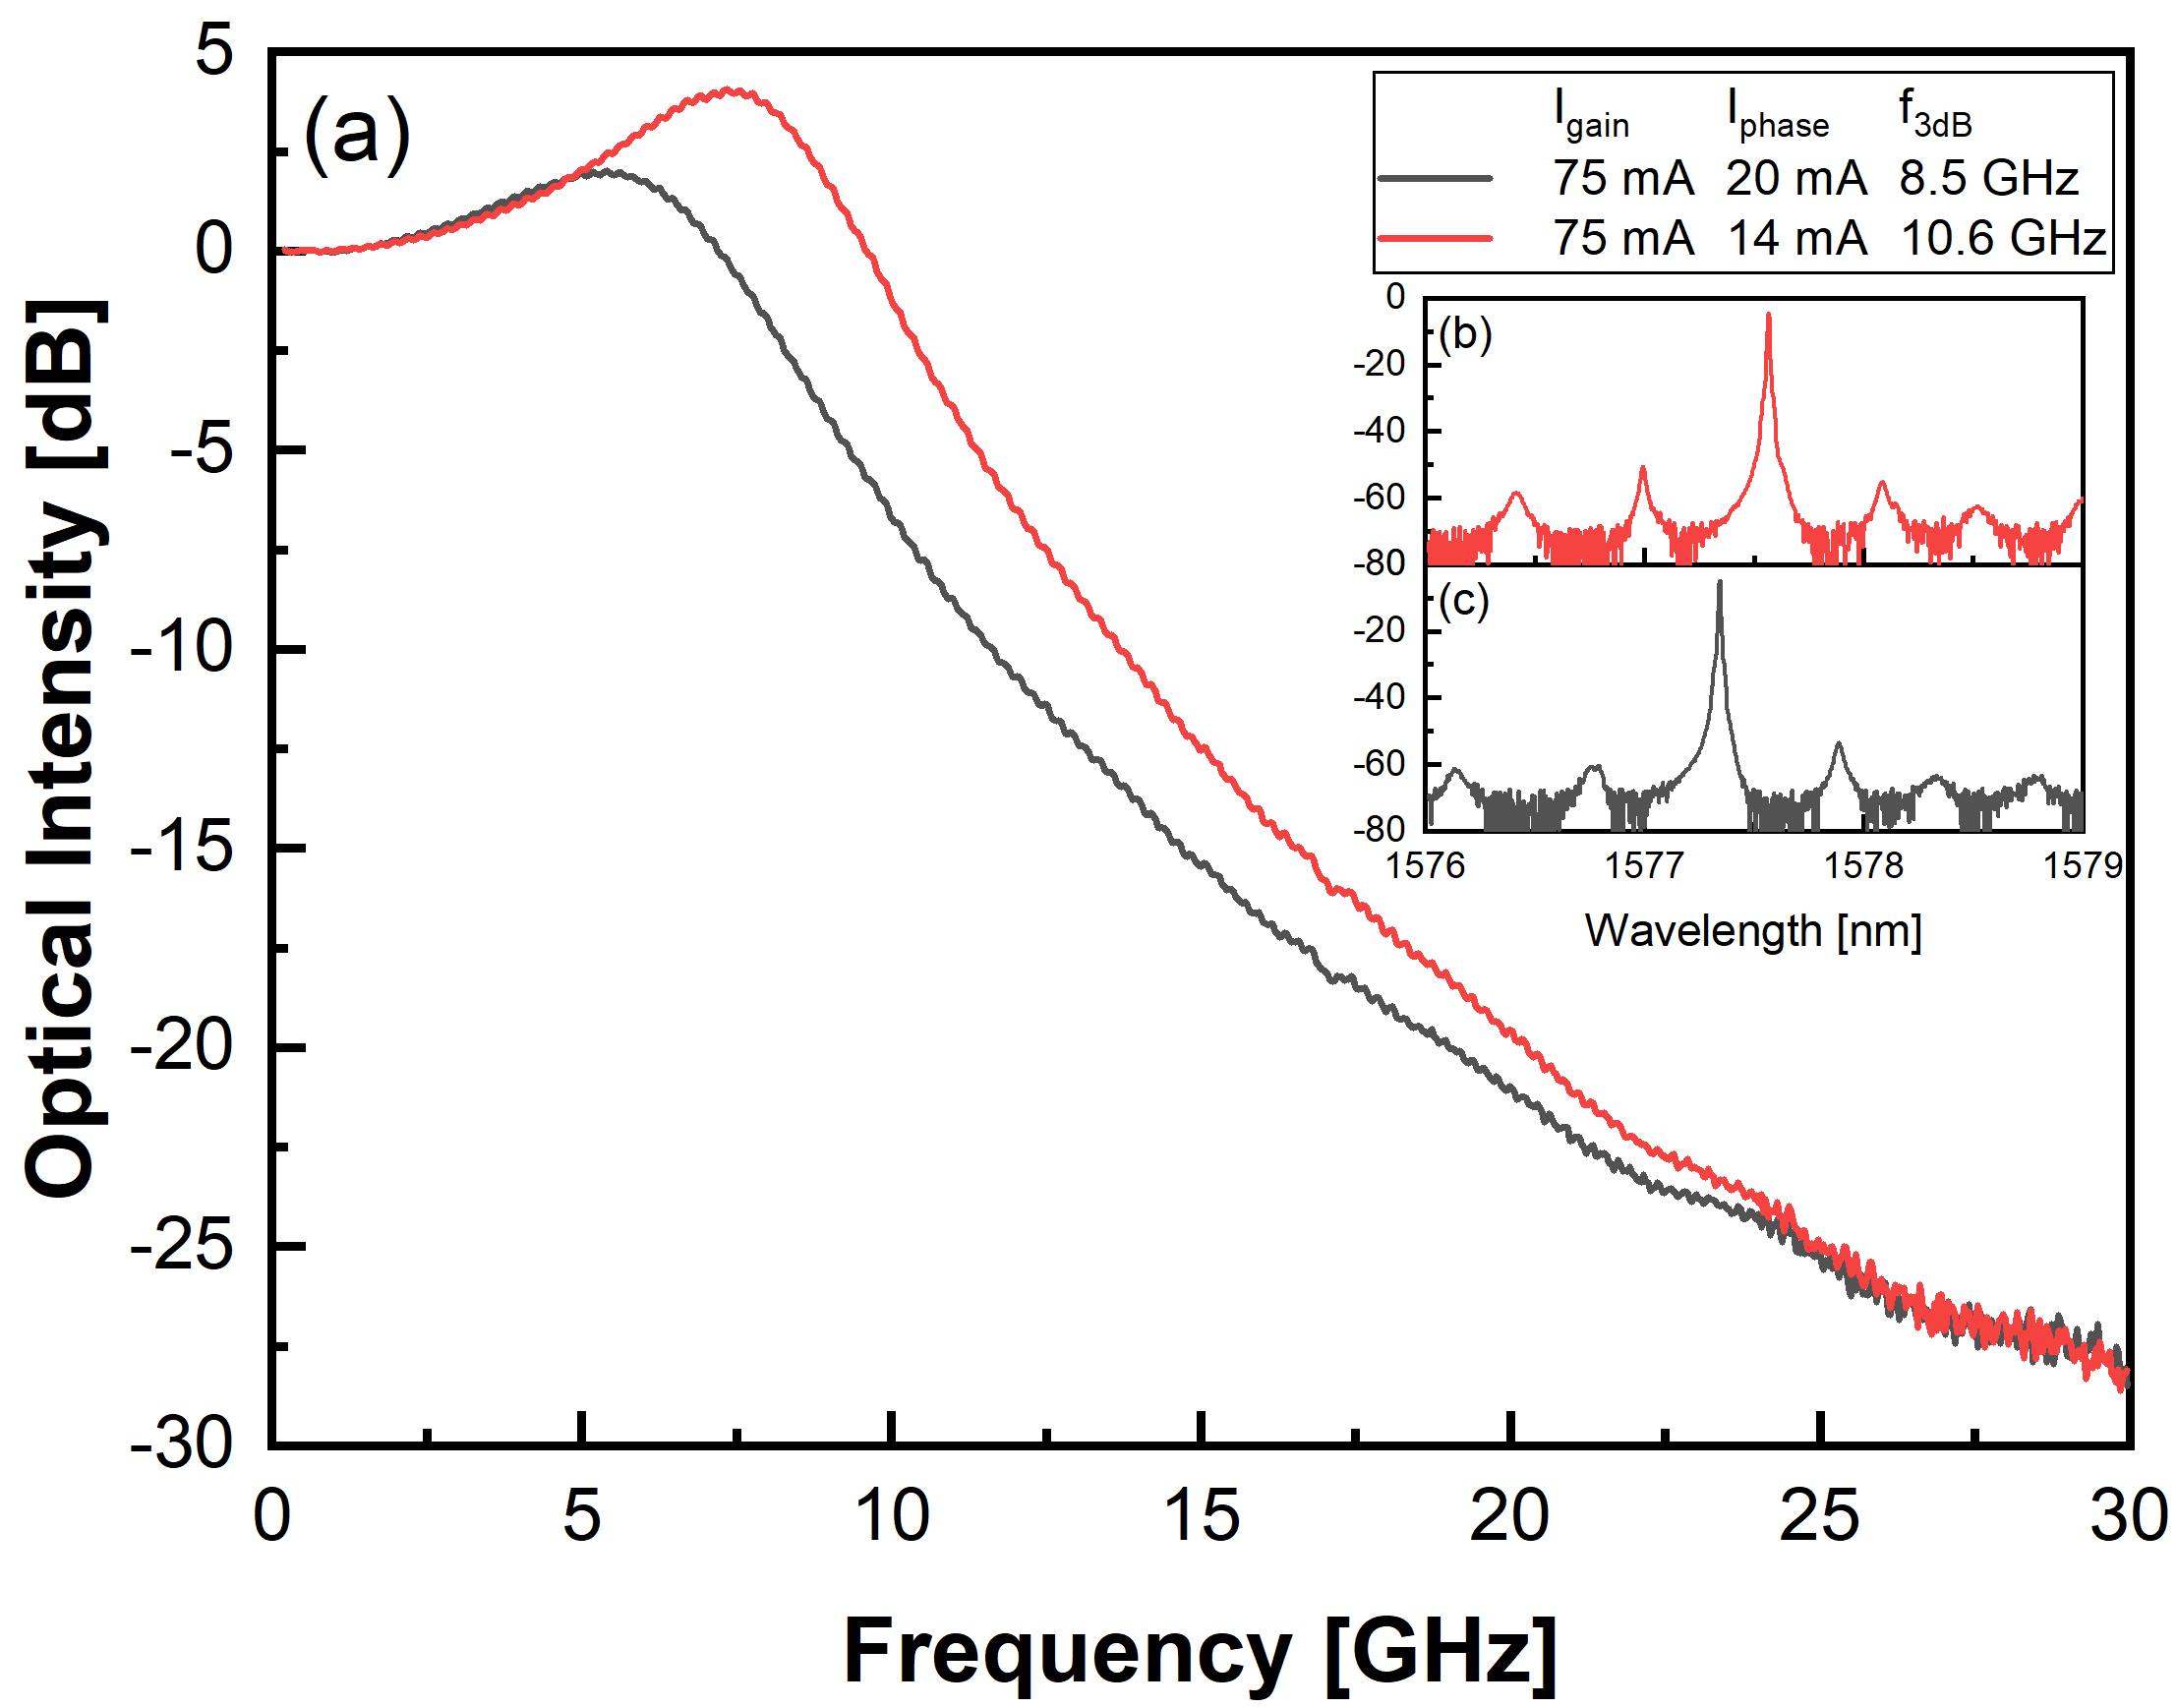
\includegraphics[width=.7\linewidth]{figures/detuned_loading.png}
%      \caption{Laser under detuned loading condition}
%      \label{fig:detuned_loading}
%   \end{minipage}
% \end{figure}

\subsection{Undamped Relaxation Oscillation}\label{subsec:undamped_RO}
Relaxation oscillation in a semiconductor laser occurs because the carrier cannot follow the photon decay rate. It usually smoothly decays out as long as the disturbance (e.g. external feedback) is small enough \cite{ohtsubo2012semiconductor}. However, it can become undamped when the laser is influenced by strong feedback (e.g. from the chip facet), which affects the laser lorentzian lineshape that the undamping peaks appear beside the main mode with the mode spacing of relaxation frequency in the spectrum. The undamped relaxation oscillation occurs for the appropriate combinations of feedback phase and strength as shown in \autoref{fig:undamped_RO_phase_scan}. The satellite peaks first show up with low phase current, then slowly increase their intensity and move towards the main peak, followed by more satellite peaks appearing when the corresponding relaxation oscillation frequency is further decreased.

\begin{figure}[ht]
    \centering
    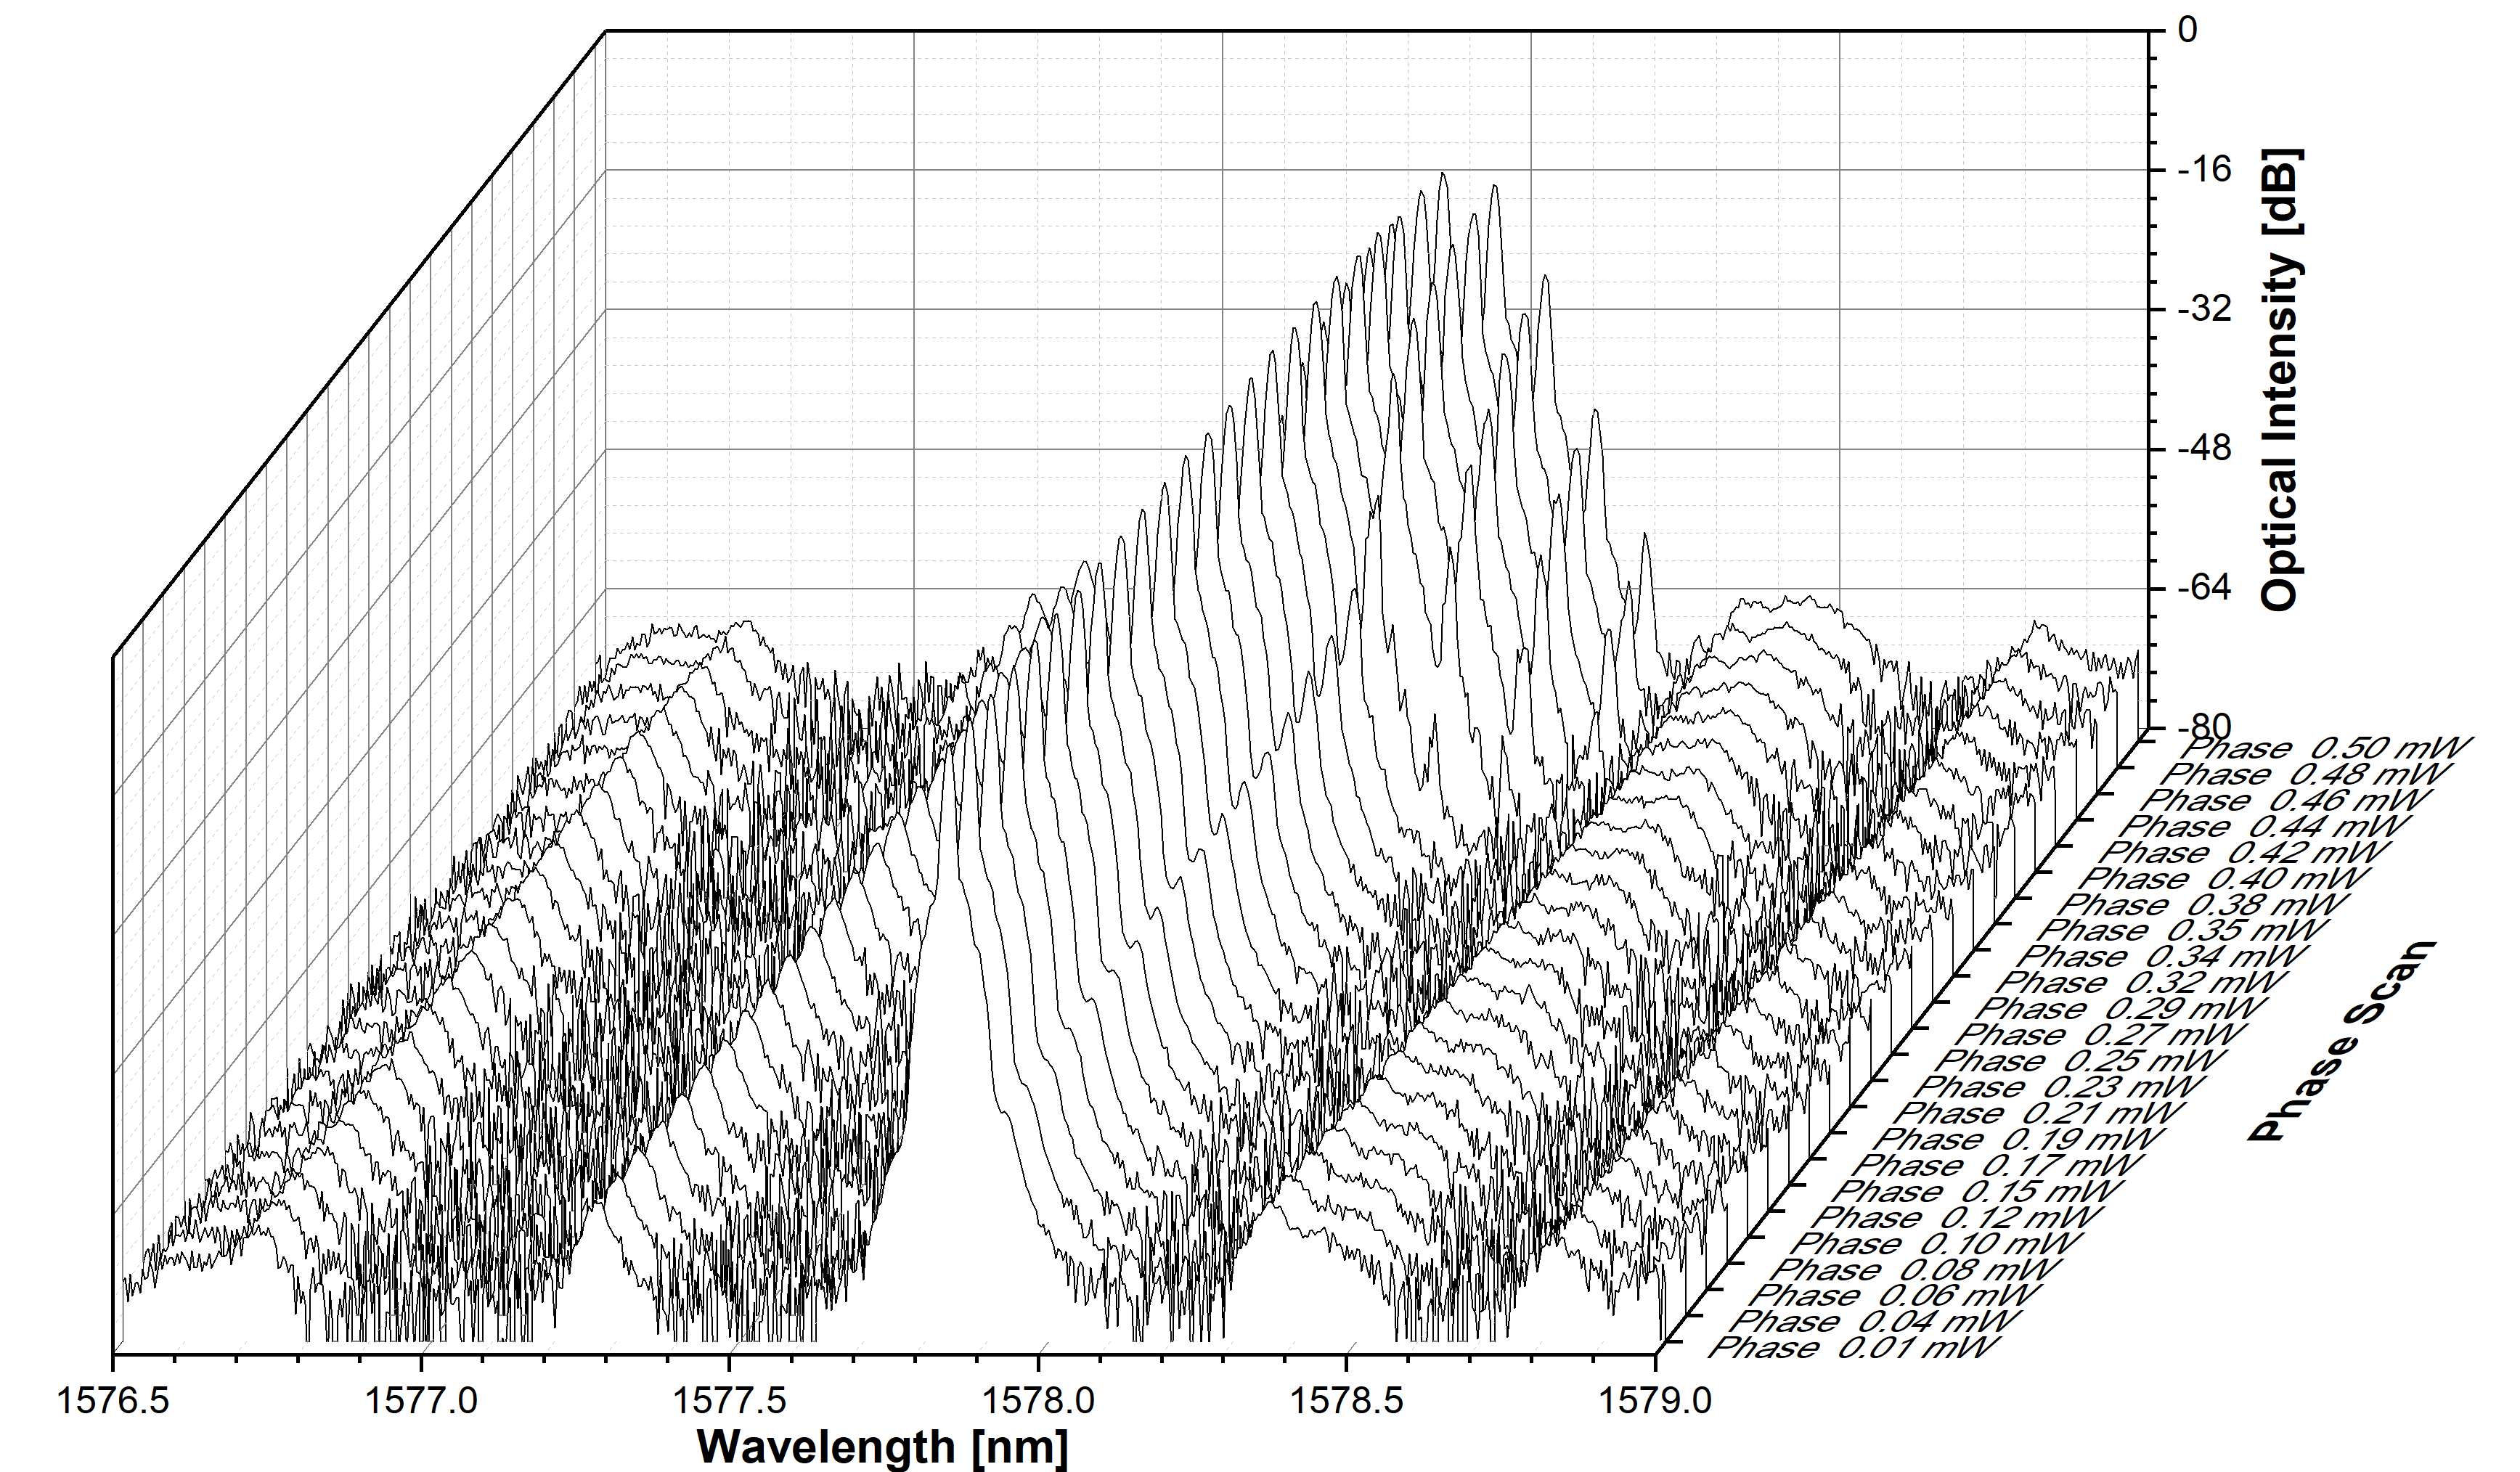
\includegraphics[width=.8\linewidth]{figures/Undamped_RO_phase_scan_grating_4621.png}
    \caption{Phase scan of the tunable DBR laser spectra with feedback from the chip facet. The side peaks of undamped RO start to appear, increase their intensity and shift toward the main peak. While the applied phase current keeps changing, more peaks develop until the laser shift to another mode and enters stable single mode lasing again.}
    \label{fig:undamped_RO_phase_scan}
\end{figure}

Since the incoming feedback acts like a perturbation for the normal laser which introduces the amplitude modulation, the undamped RO can also be called as self-modulation and self-pulsation. The mechanism of self-pulsation is analysed and discussed in \cite{bandelow1993theory} as "dispersive Q-switching". In order to explain the self-pulsations one usually assumes some kind of Q-switching process, where the term Q-switching denotes a switching of the quality-factor of the laser cavity. If an increase of optical power yields a decrease of optical loss (or an increase of optical gain) within the laser, the round trip gain may become larger than unity, yielding an exponential increase of optical power, corresponding to the rising edge of a developing pulse. On the other hand an increased power yields an increasing consumption of carriers untile finally the carrier density is too low to maintain a unity round trip gain and therefore the optical power collapses. A recovery time is required in order to increase the carrier density again until the next pulse develops. The repetition frequency for these pulses is of the same order as the relaxation resonance frequency \cite{petermann2012laser}. The bandwidth enhancement by the self-pulsation effect has beed reported as a clear undamping of the relaxation peak which in some cases ultimately led to self-pulsations at the relaxation frequency is observed in the small signal modulation response of the laser. The increased relaxation frequency and the undamping of the relaxation peak can be utilised in order to achieve higher bandwidth \cite{schatz1996enhanced}.

\subsection{Photon-Photon Resonance}\label{subsec:pp_resonance}
Another approach used to extend the dynamic properties of an integrated laser, similar to detuned loading condition, in addition takes advantage of the interaction between the lasing mode and an adjacent longitudinal cavity mode, properly separated in frequency in such a way they can interact due to the carrier pulsation introduced by the applied modulation signal at the gain section. This interaction introduces a resonance in the impulse modulation (IM) response at the frequency corresponding to the mode separation. This resonance is frequently called Photon-Photon resonance (PPR), to distinguish this interaction mechanism respect to the Carrier-Photon resonance (CPR) \cite{montrosset2014laser}. The occurence of the PPR should not be too far away from the relaxation oscillation frequency so that the dip in between two peaks will not reach the -3 dB limitation in the modulation response as shown in \autoref{fig:PP_resonance_in_modulation_response}.

\begin{figure}[ht]
    \centering
    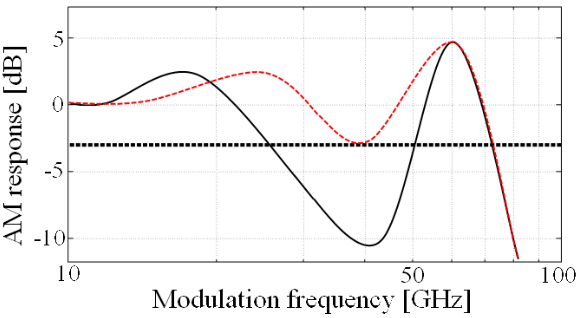
\includegraphics[width=.6\linewidth]{figures/PP_resonance_in_modulation_response.png}
    \caption{Example of modulation responses obtained in a cavity exploiting the PPR effect. The black line indicates a case in which the CPR and the PPR peaks are too far whereas in the case indicated by the red line the modulation bandwidth extension is achieved \cite{montrosset2014laser}.}
    \label{fig:PP_resonance_in_modulation_response}
\end{figure}

The large enhancement of the modulation bandwidth, already has been observed to be closely related to a special behavior of the cavity Round Trip Phase (RTP) function \cite{reithmaier2005modulation}, which is the phase factor $\varphi(\omega)$ in \autoref{eq:RTG_RTP}. In order to illustrate the operation principle of the PPR, we did the calculation by assuming the simplified DBR laser structure as in \cite{montrosset2014laser}, which contains only a gain section and a grating. Parameters used for this calculation are shown in \autoref{tab:PP_resonance_operation_principle} and the python code is provided in \autoref{sec:PP_resonance_cal}.

\begin{table}[ht]
    \centering
    \caption{Simplified DBR laser cavity parameters used for calculation \cite{montrosset2014laser}.}
    \label{tab:PP_resonance_operation_principle}
    \begin{tabular}{@{}lll@{}}
    \toprule
    Symbol    & Description                  & Value        \\ \midrule
    $L_A$     & Active region length         & 140 $\mu m$  \\
    $L_G$     & Grating region length        & 780 $\mu m$  \\
    $\kappa$  & Grating coupling coefficient & 20 $cm^{-1}$ \\
    $n_{eff}$ & Effective refractive index   & 3.7          \\
    $R_R$     & Right side reflectivity      & 0            \\
    $R_L$     & Left side reflectivity       & 0.32         \\ \bottomrule
    \end{tabular}
\end{table}

\begin{figure}[ht]
    \centering
    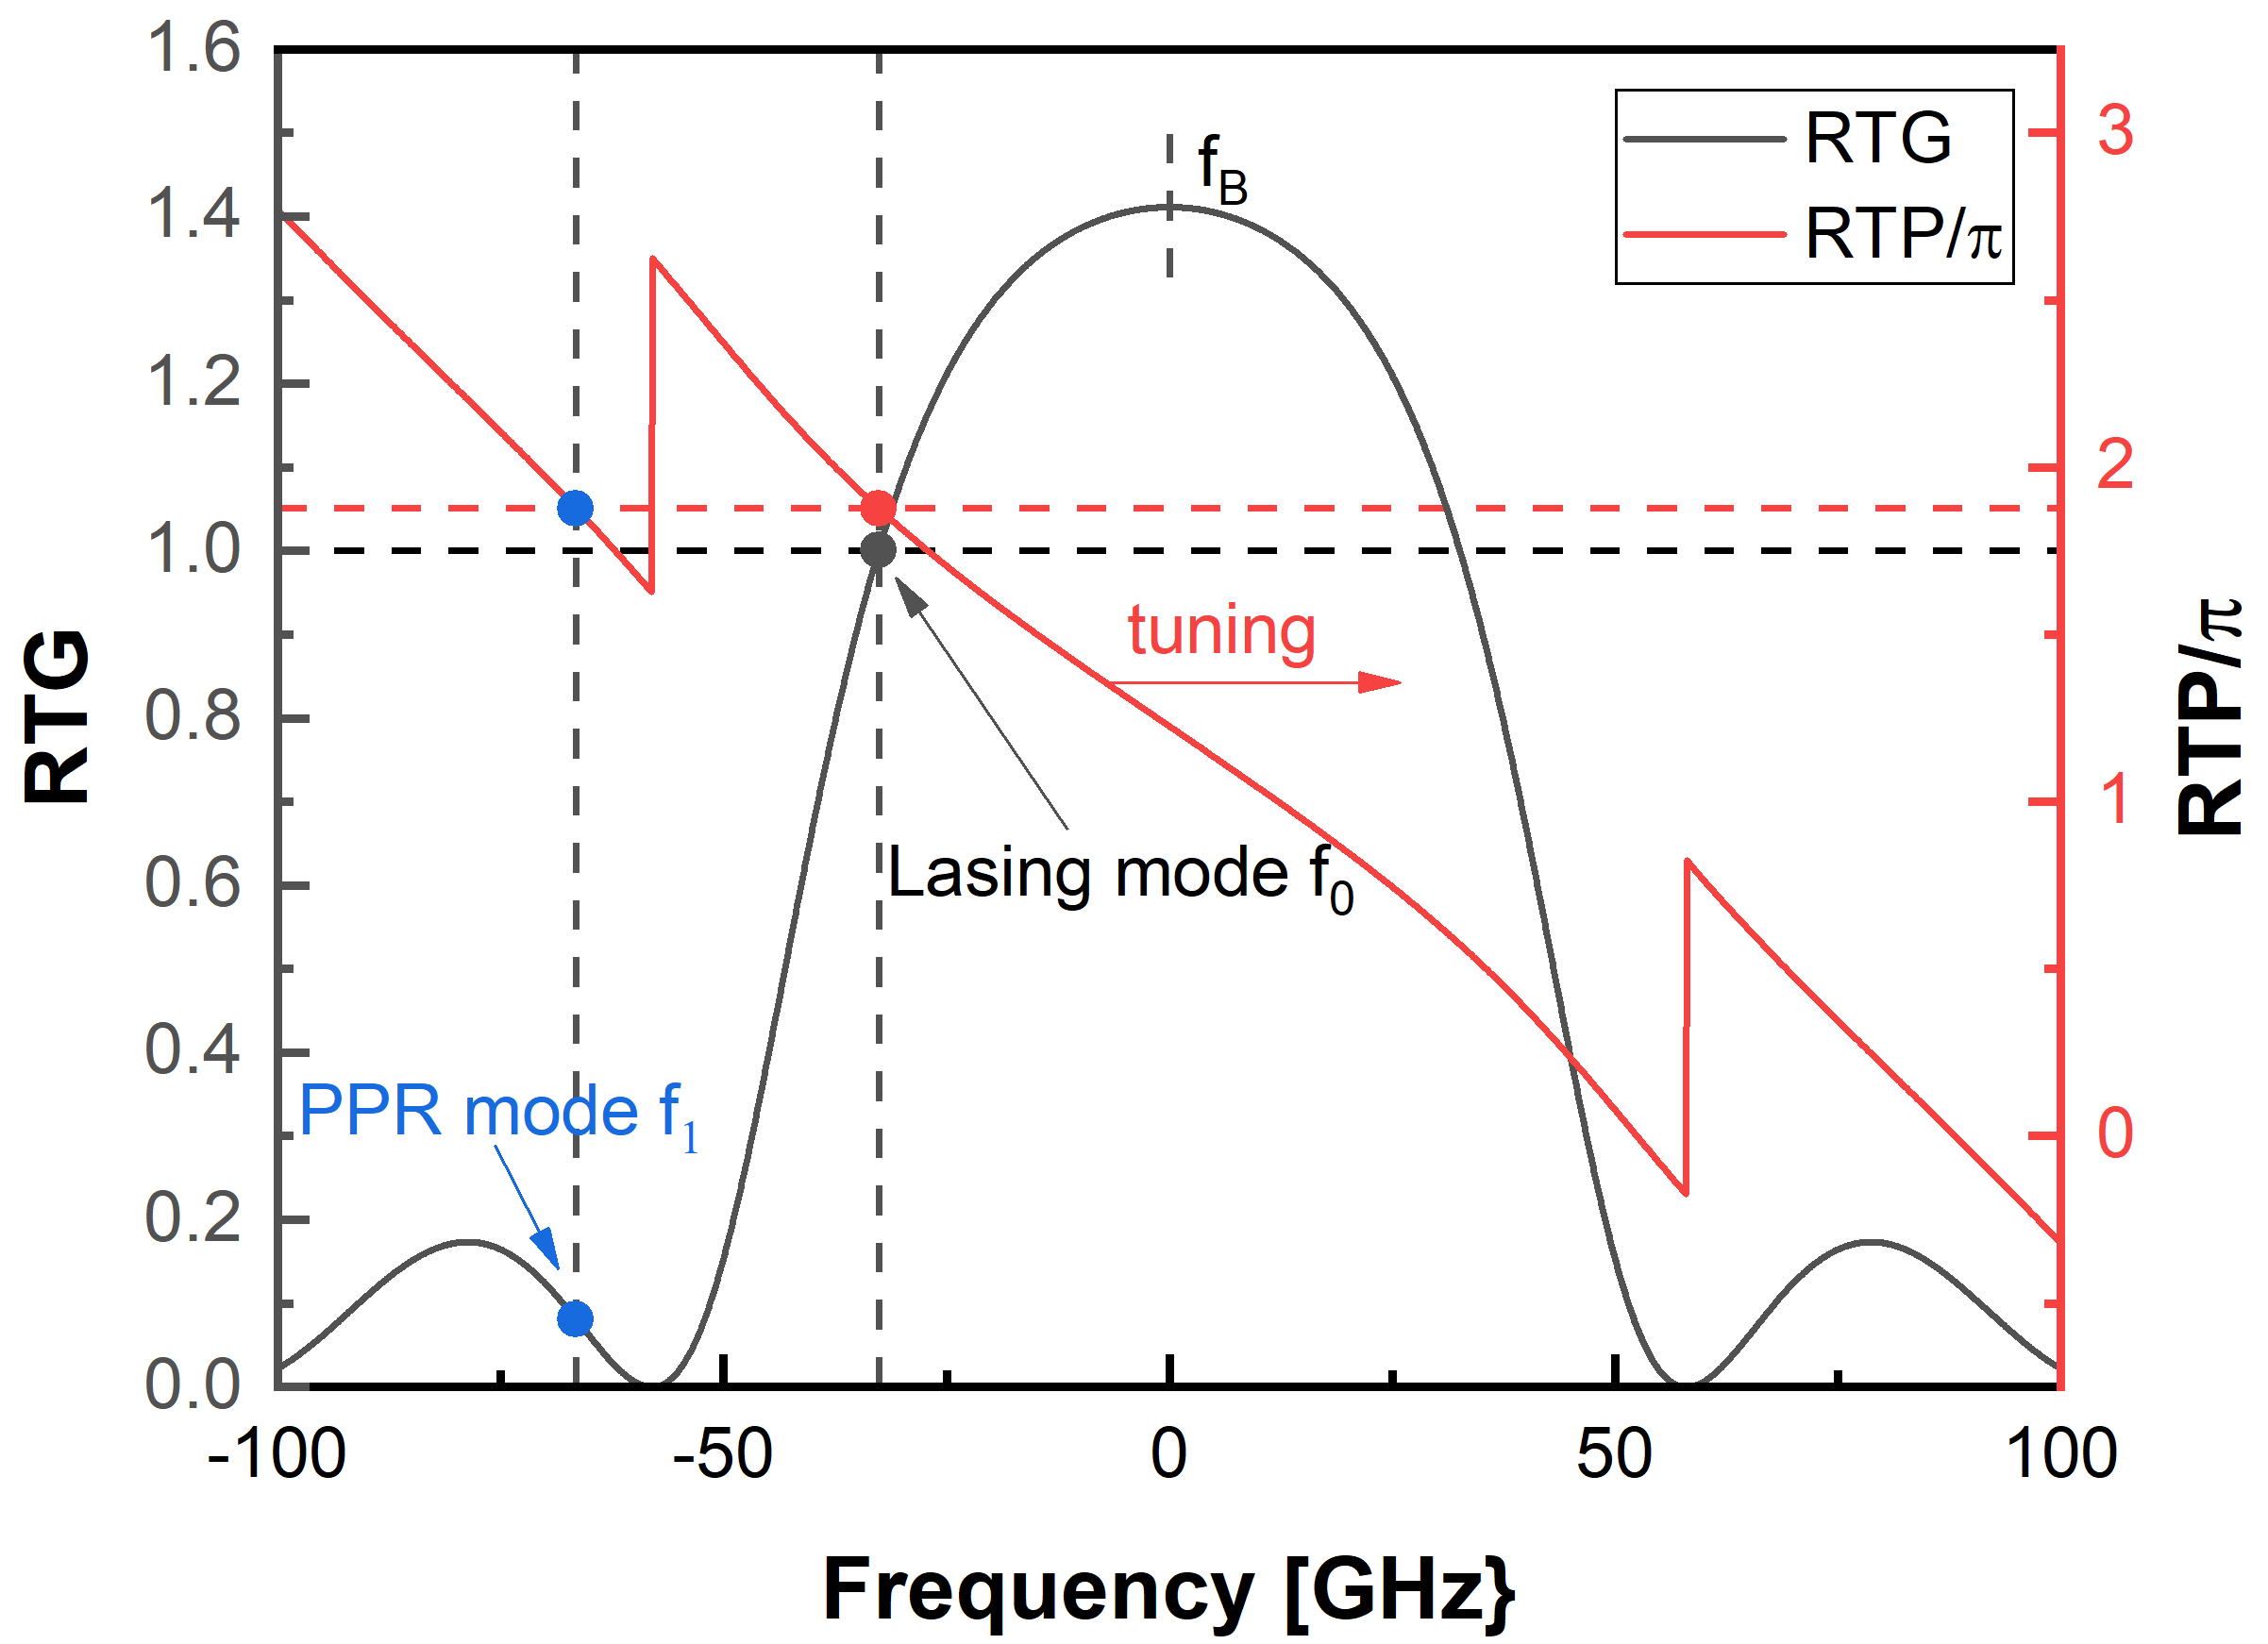
\includegraphics[width=.7\linewidth]{figures/PP_resonance_operation_principle_2.png}
    \caption{Round trip gain (RTG, grey curve) and phase (RTP, red curve) functions computed at the DBR threshold. The grey and red marker represent the lasing mode $f_0$ at the corresponding RTG and RTP curve, the blue marker indicates the PPR mode $f_1$.}
    \label{fig:PP_resonance_operation_principle}
\end{figure}

The caculated result is shown in \autoref{fig:PP_resonance_operation_principle}, from which we can see the most favorable operation condition is when the lasing mode $f_0$ operates in the detuned loaidng condition $f_0<f_B$ and a mode $f_1$ on the same side with respect to the Bragg wavelength is placed on the the first lobe of the Round Trip Gain (RTG) curve. In this mode configuration, the PPR effect can arise due to the coupling between mode $f_0$ and $f_1$ \cite{montrosset2014laser}, the corresponding PPR frequency is then the difference between the lasing mode $f_0$ and the PPR mode $f_1$. In order to generate an adjacent longitudinal cavity mode under feedback, a strong feedback condition is required, which will form compound cavity modes with the Free Spectral Range (FSR) considering the normal cavity plus the external cavity as defined in \autoref{eq:mode_spacing}
\begin{equation}
    \Delta\nu=\frac{c}{2(n_{gain}L_{gain}+n_{poly}L_{eff})}
    \label{eq:mode_spacing}
\end{equation}
this equation is also used as the design guideline in \autoref{sec:design}.

\chapter{Tunable Laser with Feedback from Chip Facet}\label{ch:Normal_laser}
Characterization of the normal tunbale DBR laser linewidth, RIN, bandwidth, $\alpha$ parameter and phase noise are measured with (1) Cleaved fiber with oil and (2) Lensed fiber, which corresponding to the laser without feedback and with feedback from chip facet conditions. Principle of each measurement will be introduced and the results will be compared in the following sections.

The measurements are done by fixing the gain section current at $I_{gain}=80 \ mA$, grating section current at $I_{grating}=15 \ mA$ and scanning the phase section from $0 \ mA$ to $30 \ mA$ with the step of $0.5 \ mA$, each current step is considered as one index which leads to in total of 61 index numbers. The principle of phase scan and the observed spectra are shown in \autoref{fig:cavity_modes_and_ext_modes_model} and \autoref{fig:spectra_lensed_4621}. By tuning the phase through the increasing current it shifts the cavity modes towards the shorter wavelength side, this effect is achieved by change of the effective refractive index inside the polymer waveguide which in turn changes the effecitve optical length of the cavity. 

\begin{figure}[ht]
    \centering
    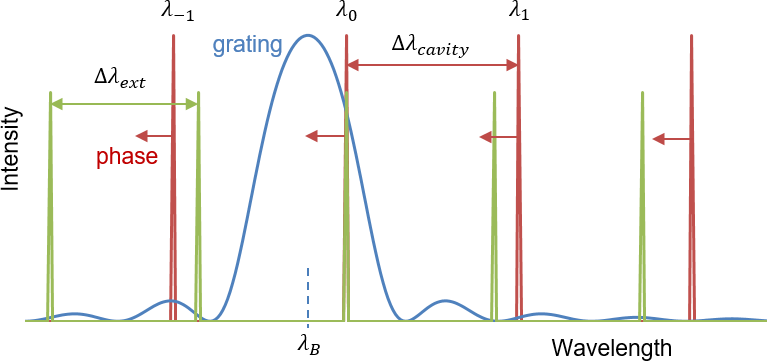
\includegraphics[width=.7\linewidth]{figures/cavity_modes_and_ext_modes_model.png}
    \caption{Principle of phase scan in tunable DBR laser. Red and green curves represent the mode of the normal cavity and external cavity respectively. The different intensity is under the consideration that usually the feedback power is less than the output power. $\lambda_0$ is the lasing mode, $\lambda_{-1}$ and $\lambda_{1}$ are its adjacent modes. $\lambda_B$ is the Bragg wavelength which indicates the center of the grating response. $\Delta\lambda_{cavity}$ and $\Delta\lambda_{ext}$ are the mode spacing of the normal cavity and the external cavity. The red arrow indicates the phase shifts the cavity modes toward the shorter wavelength through the increasing phase current. }
    \label{fig:cavity_modes_and_ext_modes_model}
\end{figure}

The scanning of the spectra and the examing of the Side Mode Suppression Ratio (SMSR) are shown in \autoref{fig:OSA_and_SMSR}. Due to the hysteresis effect the laser wavelength has a little shift under these two configurations, e.g. the mode hopping point in \autoref{fig:OSA_and_SMSR} a) appears at index 51 and the correspoinding point in \autoref{fig:OSA_and_SMSR} (b) is at index 48. Besides, the additional hopping behavior in \autoref{fig:OSA_and_SMSR} (b) is due to the feedback effect since the undamped RO peaks appearing in the spectra. Important to note that the light grey points marked at the beginning of \autoref{fig:OSA_and_SMSR} (c) are unstable working points with SMSR lower than 40 dB, several modes appeared at these phase currents and the laser performance dropped drastically, which can be seen from the $\alpha$ parameter measurement in \autoref{sec:chirp_measurement}.

\begin{figure}[ht]
    \centering
    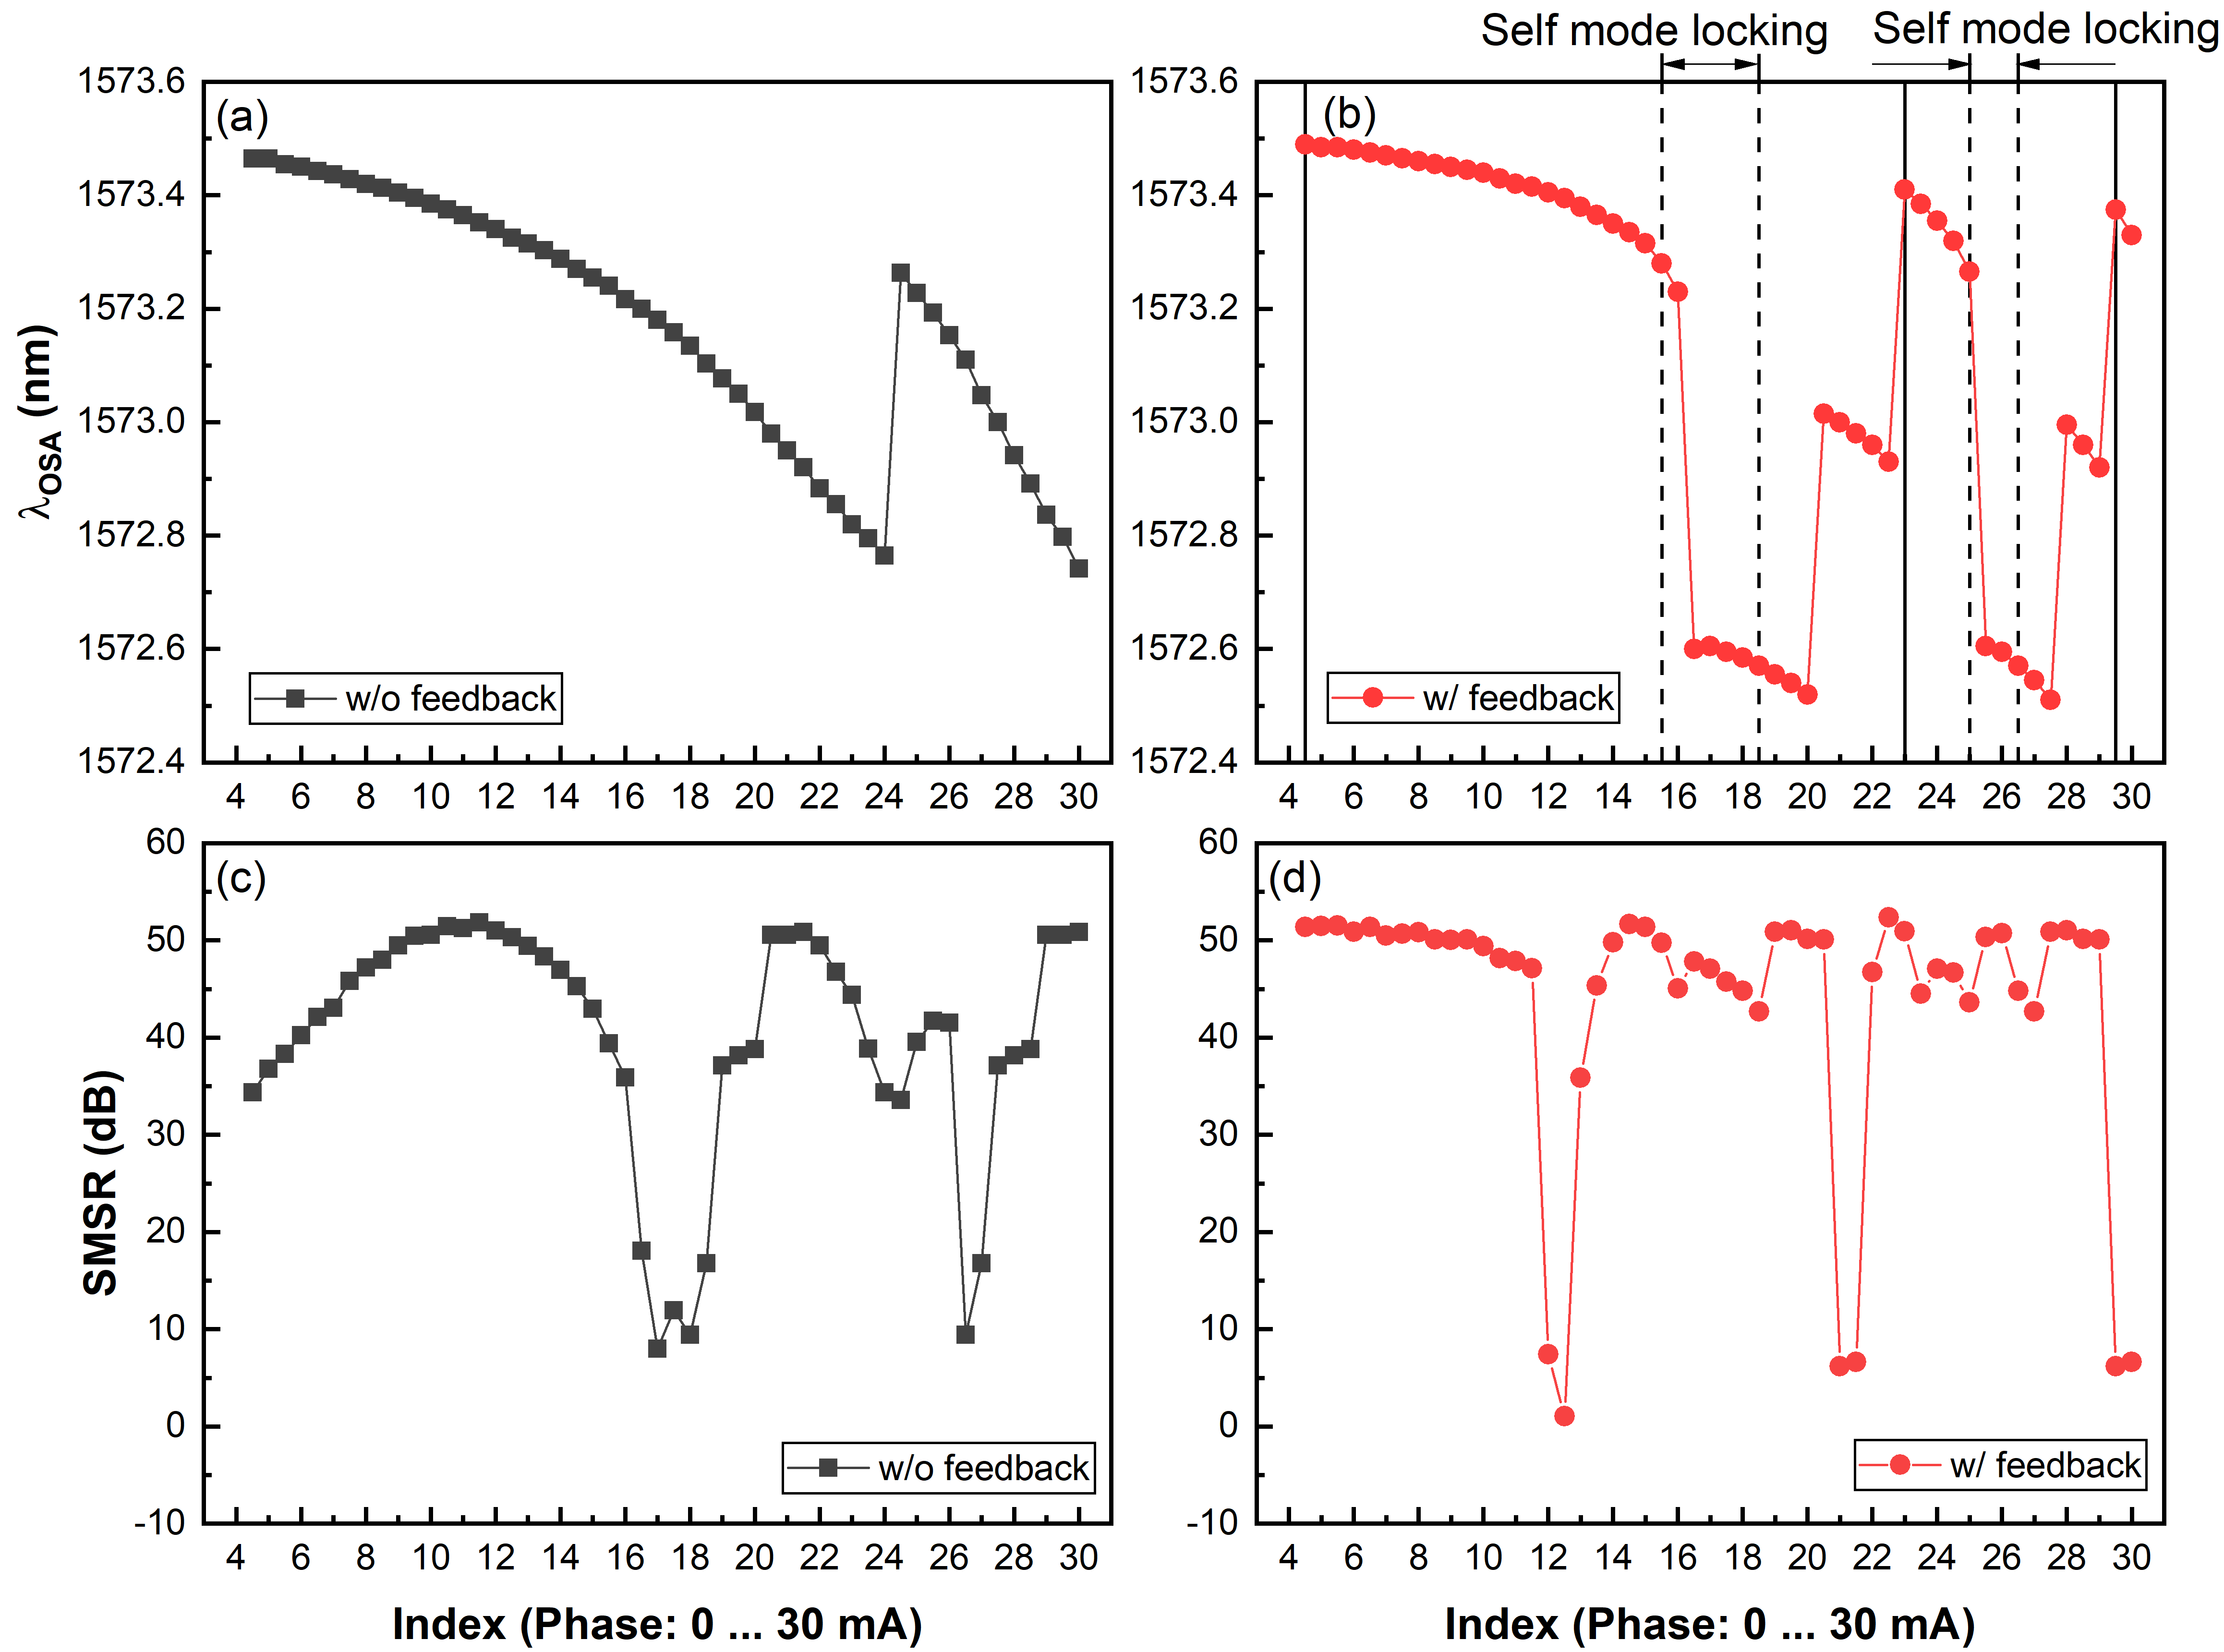
\includegraphics[width=\linewidth]{figures/OSA_and_SMSR.png}
    \caption{Comparison of wavelength scanning (a), (b) and SMSR (c), (d) for tunbale DBR laser with feedback (red circled curve) and without feedback (black squared curve). (c) The light grey squared points at the beginning are unstable working points with several modes appearing and the laser performance dropped drastically. The other points which are lower than 40 dB are corresponding to the mode hopping behavior in the wavelength scan maps.}
    \label{fig:OSA_and_SMSR}
\end{figure}

By using the parameters in \autoref{tab:F_reduction_factor} along with the external cavity formed between the end of the grating and the chip facet $L_{ext}=1473.36 \ \mu m$, we caculated the mode spacing for normal cavity and external cavaity as $\Delta\nu_{cavity}=67.04 \ GHz$ and $\Delta\nu_{ext}=56.35 \ GHz$ respectively. As seen from \autoref{fig:spectra_lensed_4621} (a), the laser initially operates with the side mode of the external cavity, it is because with the feedback from the chip facet, the laser operates in the relative strong feedback region with $C=1.69$. While shifting the phase current, the undamped RO starts to appear as shown in \autoref{fig:undamped_RO_phase_scan} and \autoref{fig:spectra_lensed_4621} (b).

\begin{figure}[ht]
    \centering
    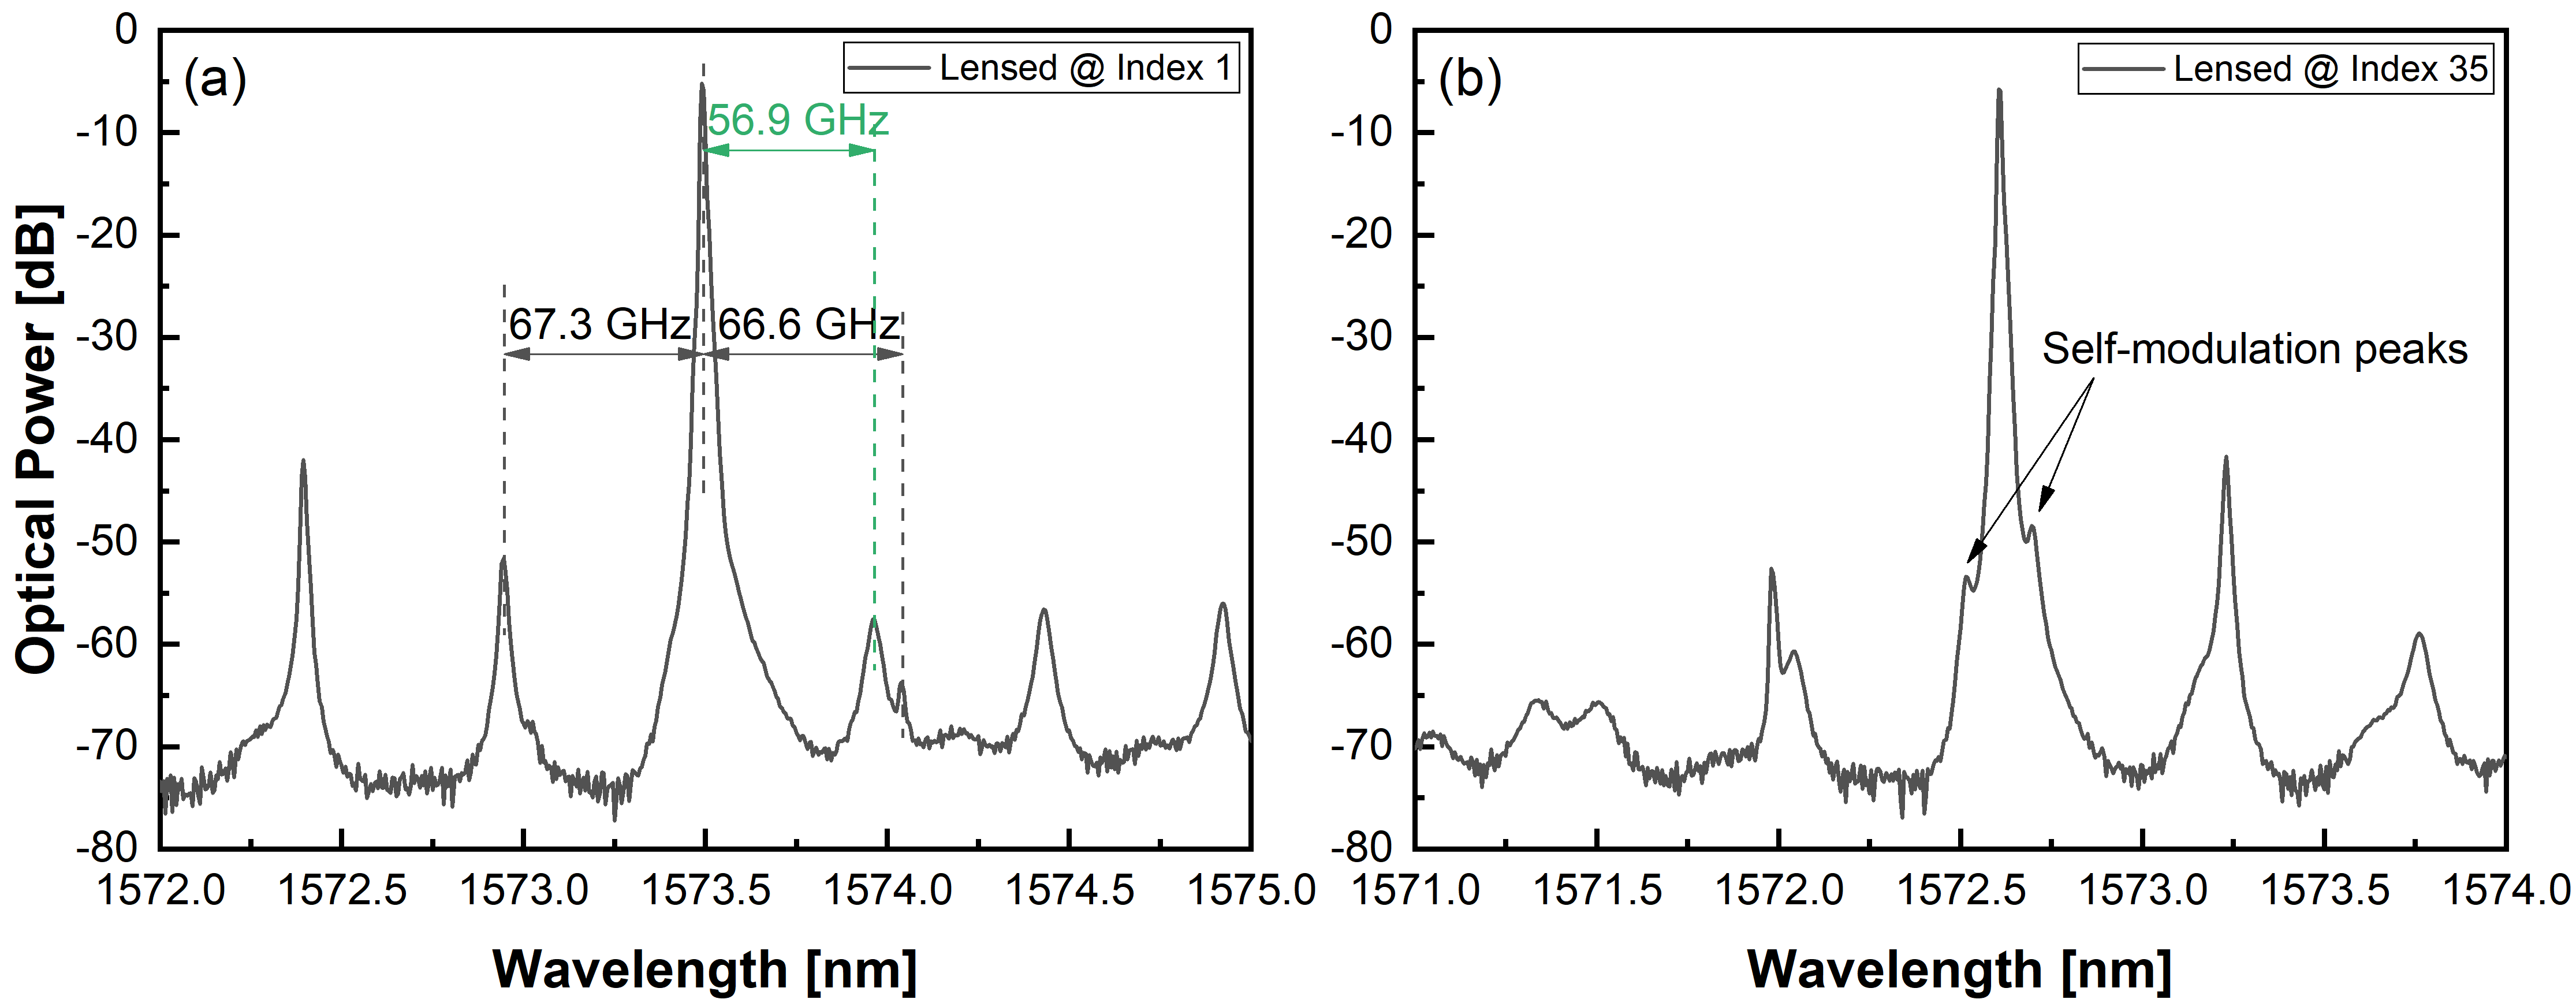
\includegraphics[width=\linewidth]{figures/spectra_lensed_4621.png}
    \caption{Example of observed spectra for different phase current (index). (a) Green dashed line indicates the mode spacing between the main mode and the first side mode on the right, which corresponds to the normal cavity mode spacing $\Delta\nu_{ext}=56.35 \ GHz$, black dashed line indicates the mode spacing correspoinds to the external cavity $\Delta\nu_{cavity}=67.04 \ GHz$, (b) occurence of the self-modulation peaks on both sides of the main mode are pointed with black arrows.}
    \label{fig:spectra_lensed_4621}
\end{figure}

Regarding to the cavity mode shifting behavior, we think the occurence of the self modulation peaks can be understood as a self mode locking behavior between the cavity mode and the external cavity mode, which is reported in \cite{tager1994high}. In our case, we use this term to name the region where the undamped RO occurs, which is marked in \autoref{fig:OSA_and_SMSR} (b), to seperate with the other lasing conditions along the phase shifting current.

\section{Linewidth Measurement}\label{sec:linewidth_measurement}
Laser linewidth is measured by self-homodyne method in the characterization. Self-homodyning can be described mathematically as a single-delay autocorrelation, which is shown in \autoref{fig:self-homodyne}, the optical spectrum at $f_0$ autocorrelates with the delayed version of itself to produce a time-fluctuating spectrum, whose detected voltage has a power spectrum centered at zero frequency. For the case of a laser with Lorentzian lineshape, the half-width of the detected spectrum is equal to the linewidth of the laser.
\begin{figure}[ht]
    \centering
    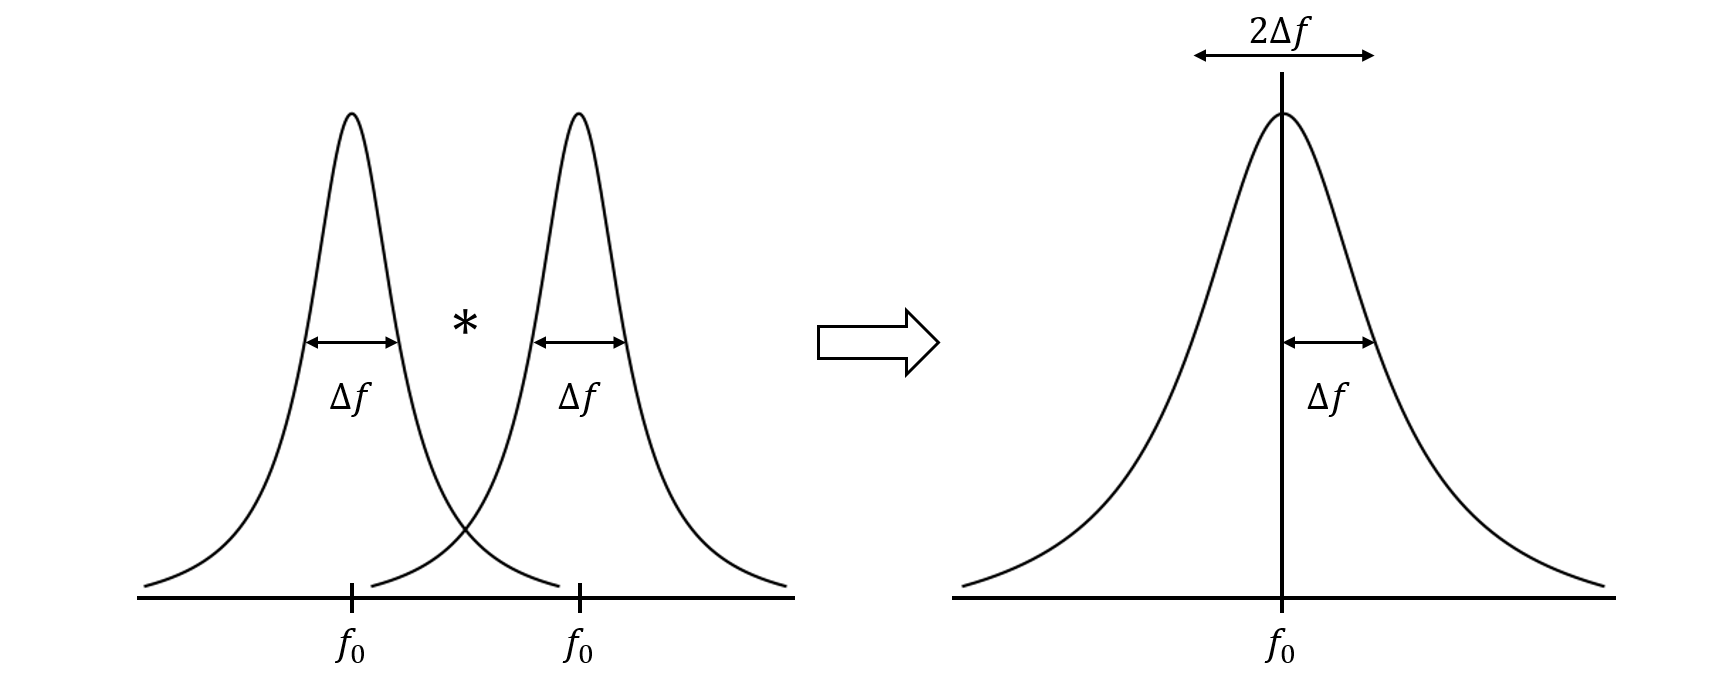
\includegraphics[width=.8\linewidth]{figures/self-homodyne.png}
    \caption{Linewidth of a DBR laser using the self-homodyne technique. The optical spectrum at $f_0$ autocorrelates with the delayed version of itself to produce a time-fluctuating spectrum, whose detected voltage has a power spectrum centered at zero frequency, the half-width of the detected spectrum is equal to the linewidth of the laser.}
    \label{fig:self-homodyne}
\end{figure}

The self-homodyne measurement set-up is shown in \autoref{fig:self-homodyne_setup}. The input directional coupler of the interferometer splits the light from the laser into two paths. One path is delayed in order to decorrelate the combinning signals, $P_1$ and $P_2$. The output coupler combines the two signals, which are then mixed at the photodectector of the lightwave signal analyzer.  The homodyne power spectrum is then observed on the analyzer from which the Lorentzian linewidth is measured by placing a marker at the half power frequency.
\begin{figure}[ht]
    \centering
    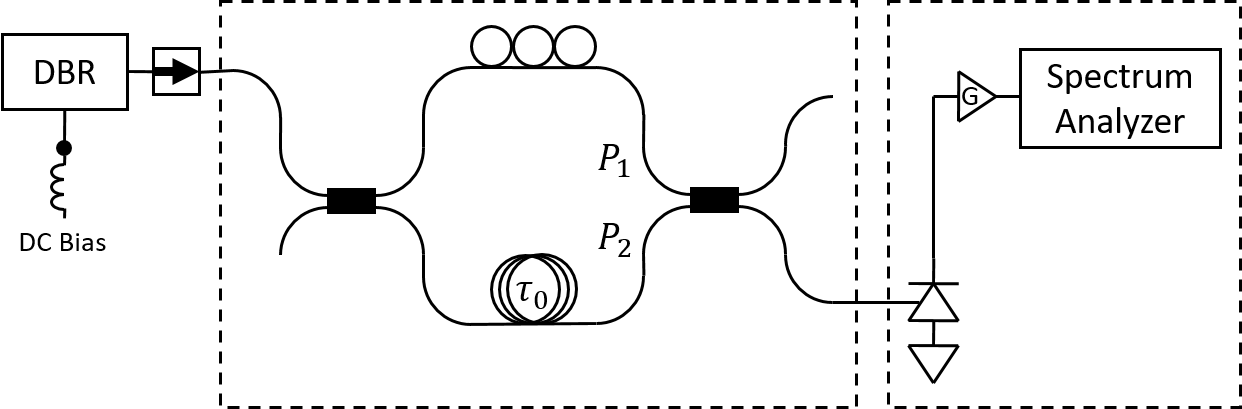
\includegraphics[width=.8\linewidth]{figures/self-homodyne_setup.png}
    \caption{Schematic set-up for self-homodyne linewidth measurement.}
    \label{fig:self-homodyne_setup}
\end{figure}

The results of linewidth measurement are shown in \autoref{fig:LB_Cleaved_and_Lensed}. Except for the unstable working points which are shown in light grey squares in \autoref{fig:LB_Cleaved_and_Lensed} (a), the laser linwidth under feedback shows a more stable transition and become narrower than the case without feedback. It is due to the reason that the external refelctor formed by the polymer/air interface with $C=1.69$ is considered to be in the relative strong feedback region. In such case, the practical formula for linewidth reduction factor $F^2$ \autoref{eq:F_strong_feedback} has to be considered. The comparison for the lowerest linewidth for two configurations, along with the theoretical predcition, is shown in \autoref{tab:linewidth_comparision}.

\begin{figure}[ht]
    \centering
    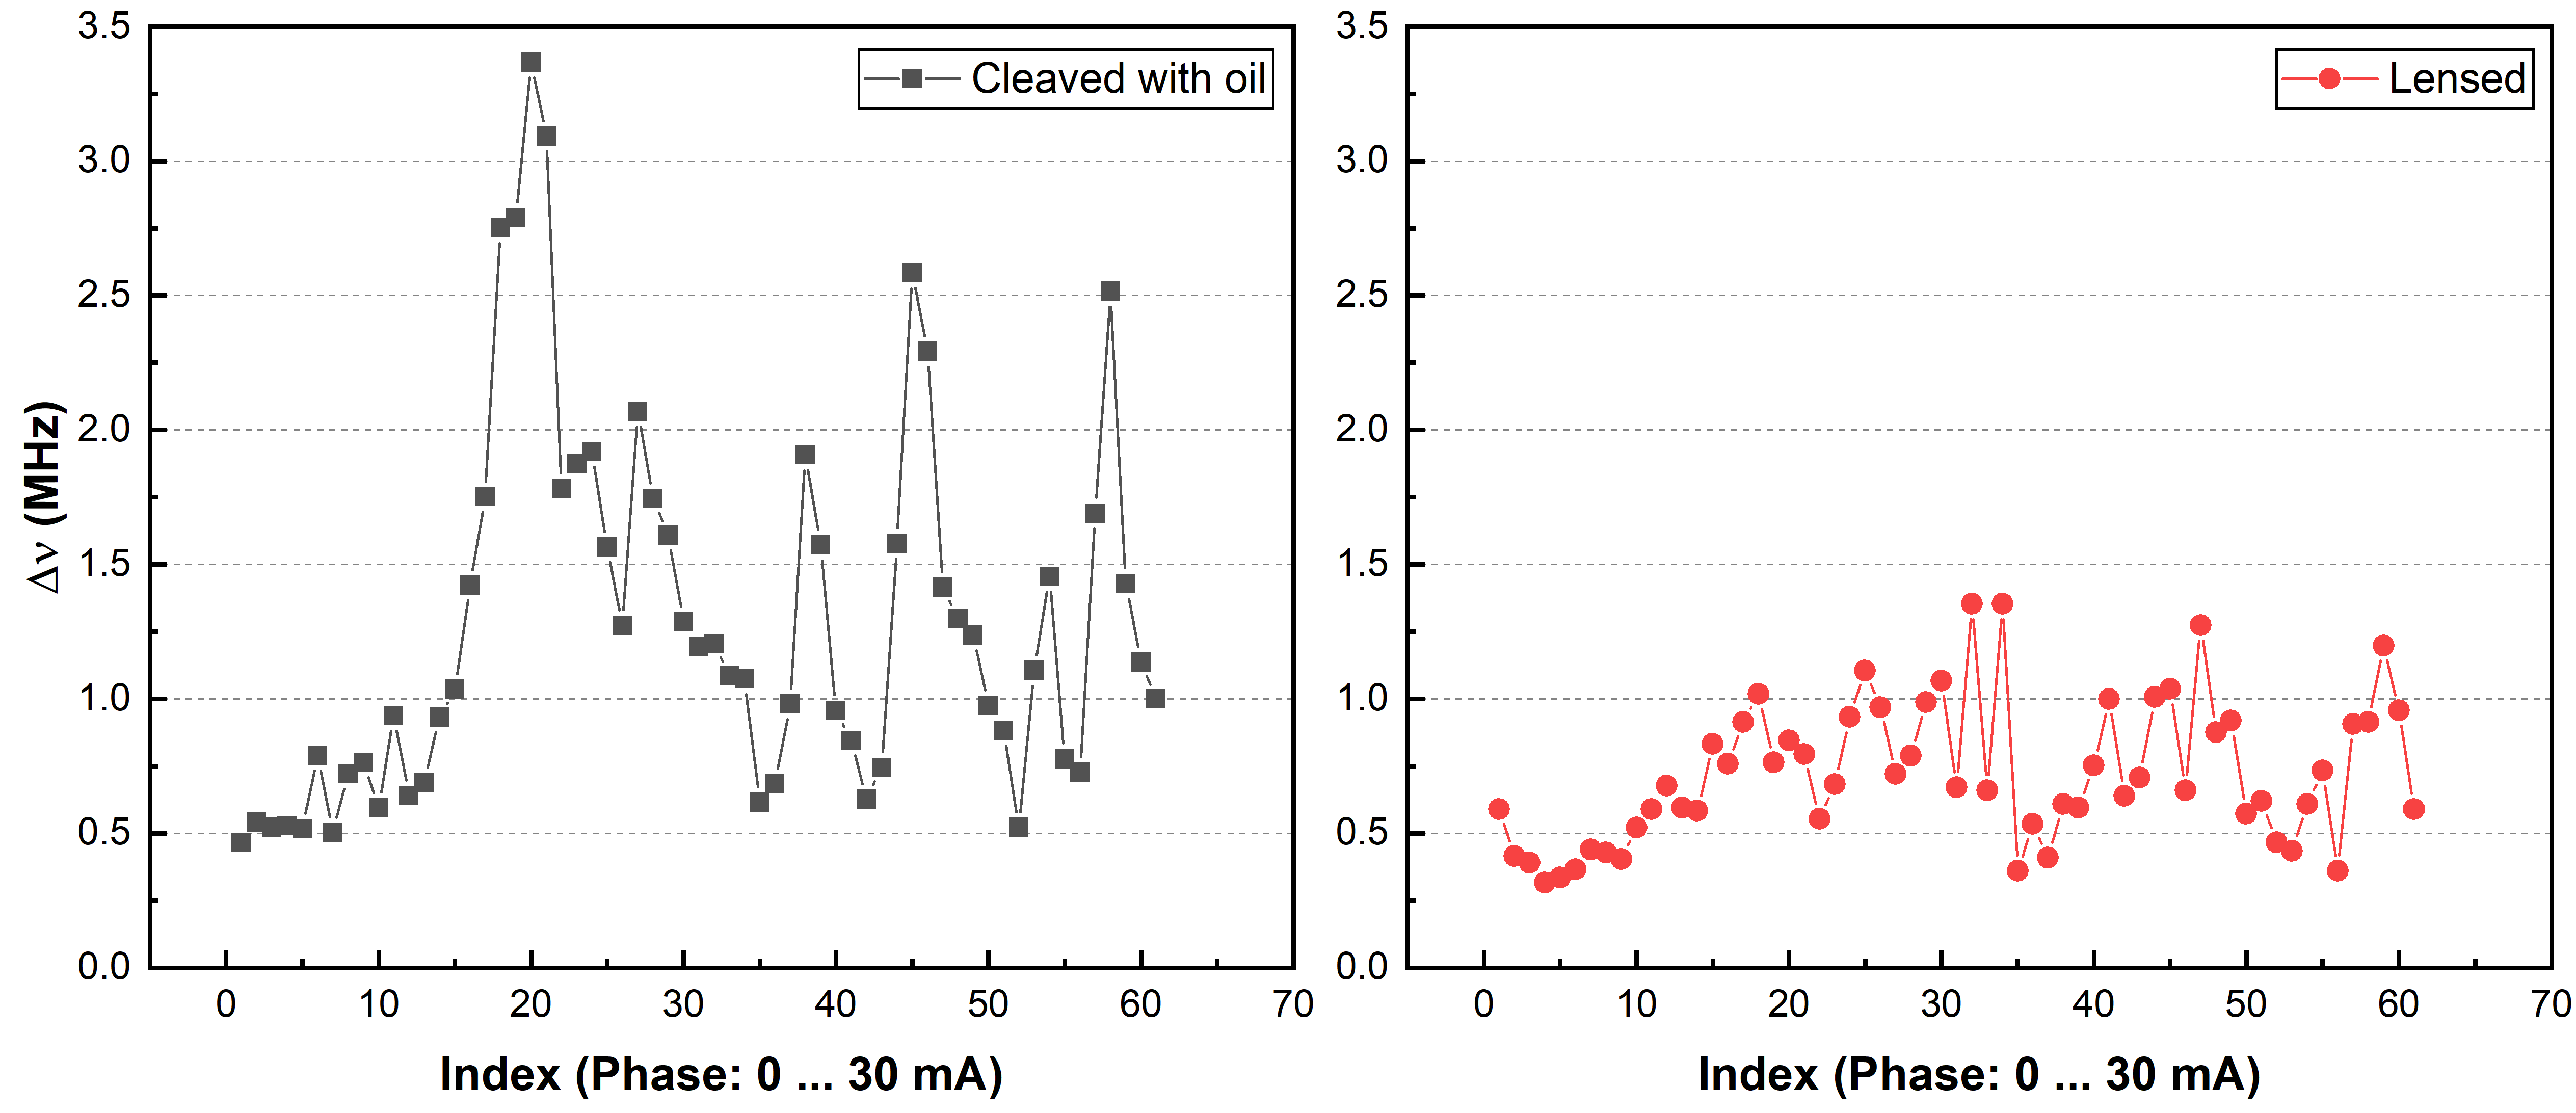
\includegraphics[width=\linewidth]{figures/LB_Cleaved_and_Lensed.png}
    \caption{(a) The laser linewidth without feedback from the chip facet, the light grey points indicate the bad working points, (b) laser linewidth with feedback from the chip facet, it appears to be more stable compare to the laser without feedback. The achieved lowest linewidth point are pointed with black arrow in each case.}
    \label{fig:LB_Cleaved_and_Lensed}
\end{figure}

\begin{table}[ht]
    \centering
    \caption{Comparison between the linewidth reduction value achieved by laser w/ and w/o feedback and the predicated reduction value.}
    \begin{tabular}{@{}lllll@{}}
    \toprule
                                             & Cleaved with oil & Lensed          & Reduction & \multicolumn{1}{c}{\begin{tabular}[c]{@{}c@{}}Reduction\\ (Predicated)\end{tabular}} \\ \midrule
    \multicolumn{1}{c}{$\Delta \nu \ (MHz)$} & 0.522 @ Index 52 & 0.317 @ Index 4 & 1.647     & 1.11                                                                                 \\ \bottomrule
    \end{tabular}
    \label{tab:linewidth_comparision}
\end{table}

\section{Relative Intensity Noise (RIN) Measurement}\label{sec:RIN_measurement}
The measurement of relative intensity noise (RIN) describes the laser’s maximum available range for signal modulation and serves as a quality indicator of laser devices. RIN is defined as the ratio of the mean-square optical intensity noise to the square of the average optical power \cite{petermann2012laser}
\begin{equation}
    RIN=\frac{\langle \Delta P \rangle ^2}{\langle P \rangle ^2}dB/Hz
\label{RIN_1}
\end{equation}
where $\langle \Delta P \rangle ^2$ is the mean-square optical intensity fluctuations (in a 1-Hz bandwidth) at a specified frequency, and $\langle P \rangle$ is the mean optical power.

In order to measure the RIN, the optical power is converted to a current after the receiving photodiode and the ratio of optical powers squared is equivalent to the ratio of the detected electrical powers. Thus, $RIN$ can be expressed in terms of detected electrical powers. \autoref{RIN_1} can be rewritten as
\begin{equation}
    RIN=\frac{N_{elec}}{P_{avg}(elec)} \ dB/Hz
    \label{eq:RIN_2}
\end{equation}
where $N_{elec}$ is the power-spectral density of the photocurrent at a specified frequency, and $P_{avg}(elec)$ is the average power of the photocurrent.

The noise at the receiver output results from three fundamental contributions: laser intensity noise primarily due to spontaneous light emissions; thermal noise from the electronics; and photonic shot noise. Since the photonic shot noise and the receiver thermal noise are not included in the definition of $N_{elec}$, they have to be subtracted from the measured $RIN$ results
\begin{equation}
    N_{laser}=N_{elec}-N_{shot}-N_{thermal} \ W/Hz
    \label{eq:RIN_3}
\end{equation}
By using \autoref{eq:RIN_2} and \autoref{eq:RIN_3}, the value of $RIN_{laser}$ can be determined
\begin{equation}
    RIN_{laser}=RIN(measured)-\frac{2e}{I_{avg}}-\frac{N_{thermal}}{P_{avg}(elec)}
    \label{eq:RIN_4}
\end{equation}
where $e$ is the elementary charge, $I_{avg}$ denotes the detected average photocurrent, $N_{thermal}$ is the measured noise floor of the lightwave signal analyzer in a 1-Hz bandwidth.

The RIN comparison for the two configurations are shown in \autoref{fig:RIN_cleaved_and_lensed}. The RIN value for laser w/o feedback ranges from $-144.086 \ dB/Hz$ to $-141.507 \ dB/Hz$ while for lase w/ feedback it has two parts: without the spikes it ranges from $-146.283 \ dB/Hz$ to $-140.216 \ dB/Hz$, which is lower than the case w/o feedback; the spikes appear in \autoref{fig:RIN_cleaved_and_lensed} (b) are correspoinding to the additional mode hopping behavior in \autoref{fig:OSA_and_SMSR} (b), which indicates the appearing of the undamped RO, will increase the RIN value.

\begin{figure}[ht]
    \centering
    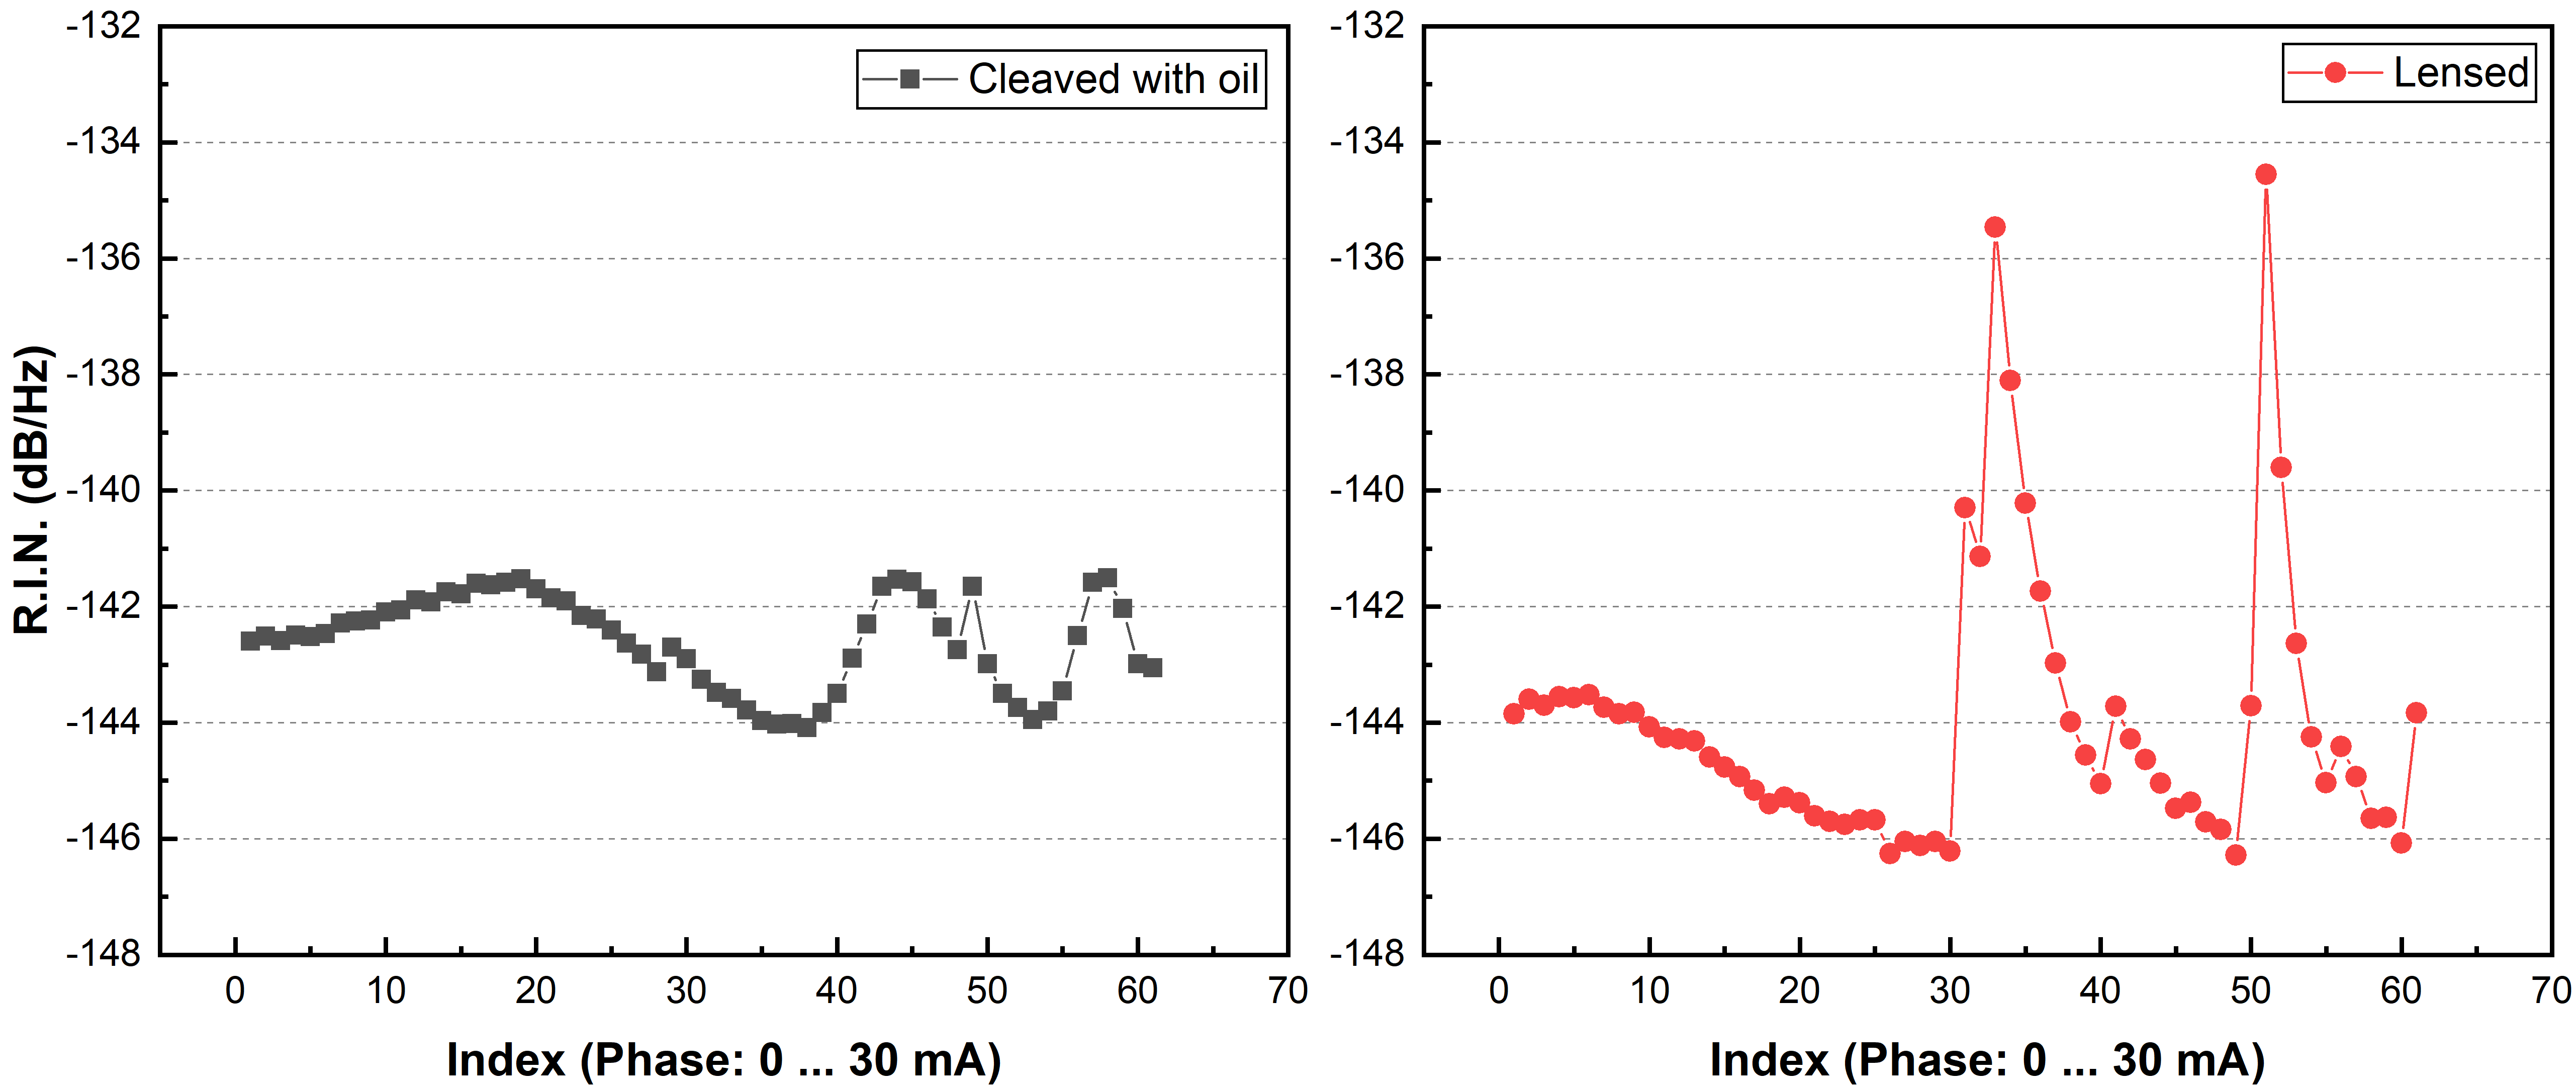
\includegraphics[width=\linewidth]{figures/RIN_cleaved_and_lensed.png}
    \caption{Comparison of the RIN value for laser w/ and w/o feedback. (a) Laser with feedback, (b) laser without feedback, the spikes indicate the appearing of the undamped RO, which increase the RIN significantly.}
    \label{fig:RIN_cleaved_and_lensed}
\end{figure}

\section{Bandwidth Measurement}\label{sec:bandwidth_measurement}
\subsection{Small Signal Modulation}
The frequency response of the laser transmitter under small signal modulation is found by the usual assumption of a harmonic current modulation superimposed on a constant bias above threshold. The modulation bandwidth $f_{3dB}$ is a measure of the maximum modulation ability in semiconductor lasers through the injection current. It is usually defined as the frequency at which the modulation response has dropped by $3 \ dB$ relative to its zero freqeuncy value \cite{ohtsubo2012semiconductor, agrawal2013semiconductor}. The characteristics of the small signal modulation are mainly determined by the relaxation oscillation frequency $f_r$, which indicated by the position of the peak in the modulation response.

% From a practical viewpoint the quantity of interest is the modulation bandwidth $\nu_B$ which indicates the frequency range over which the laser responds to the current modulation. It is usually defined as the frequency at which the modulation response has dropped by 3 dB relative to its low-frequency or DC value \cite{agrawal2013semiconductor}.
\begin{figure}[ht]
    \centering
    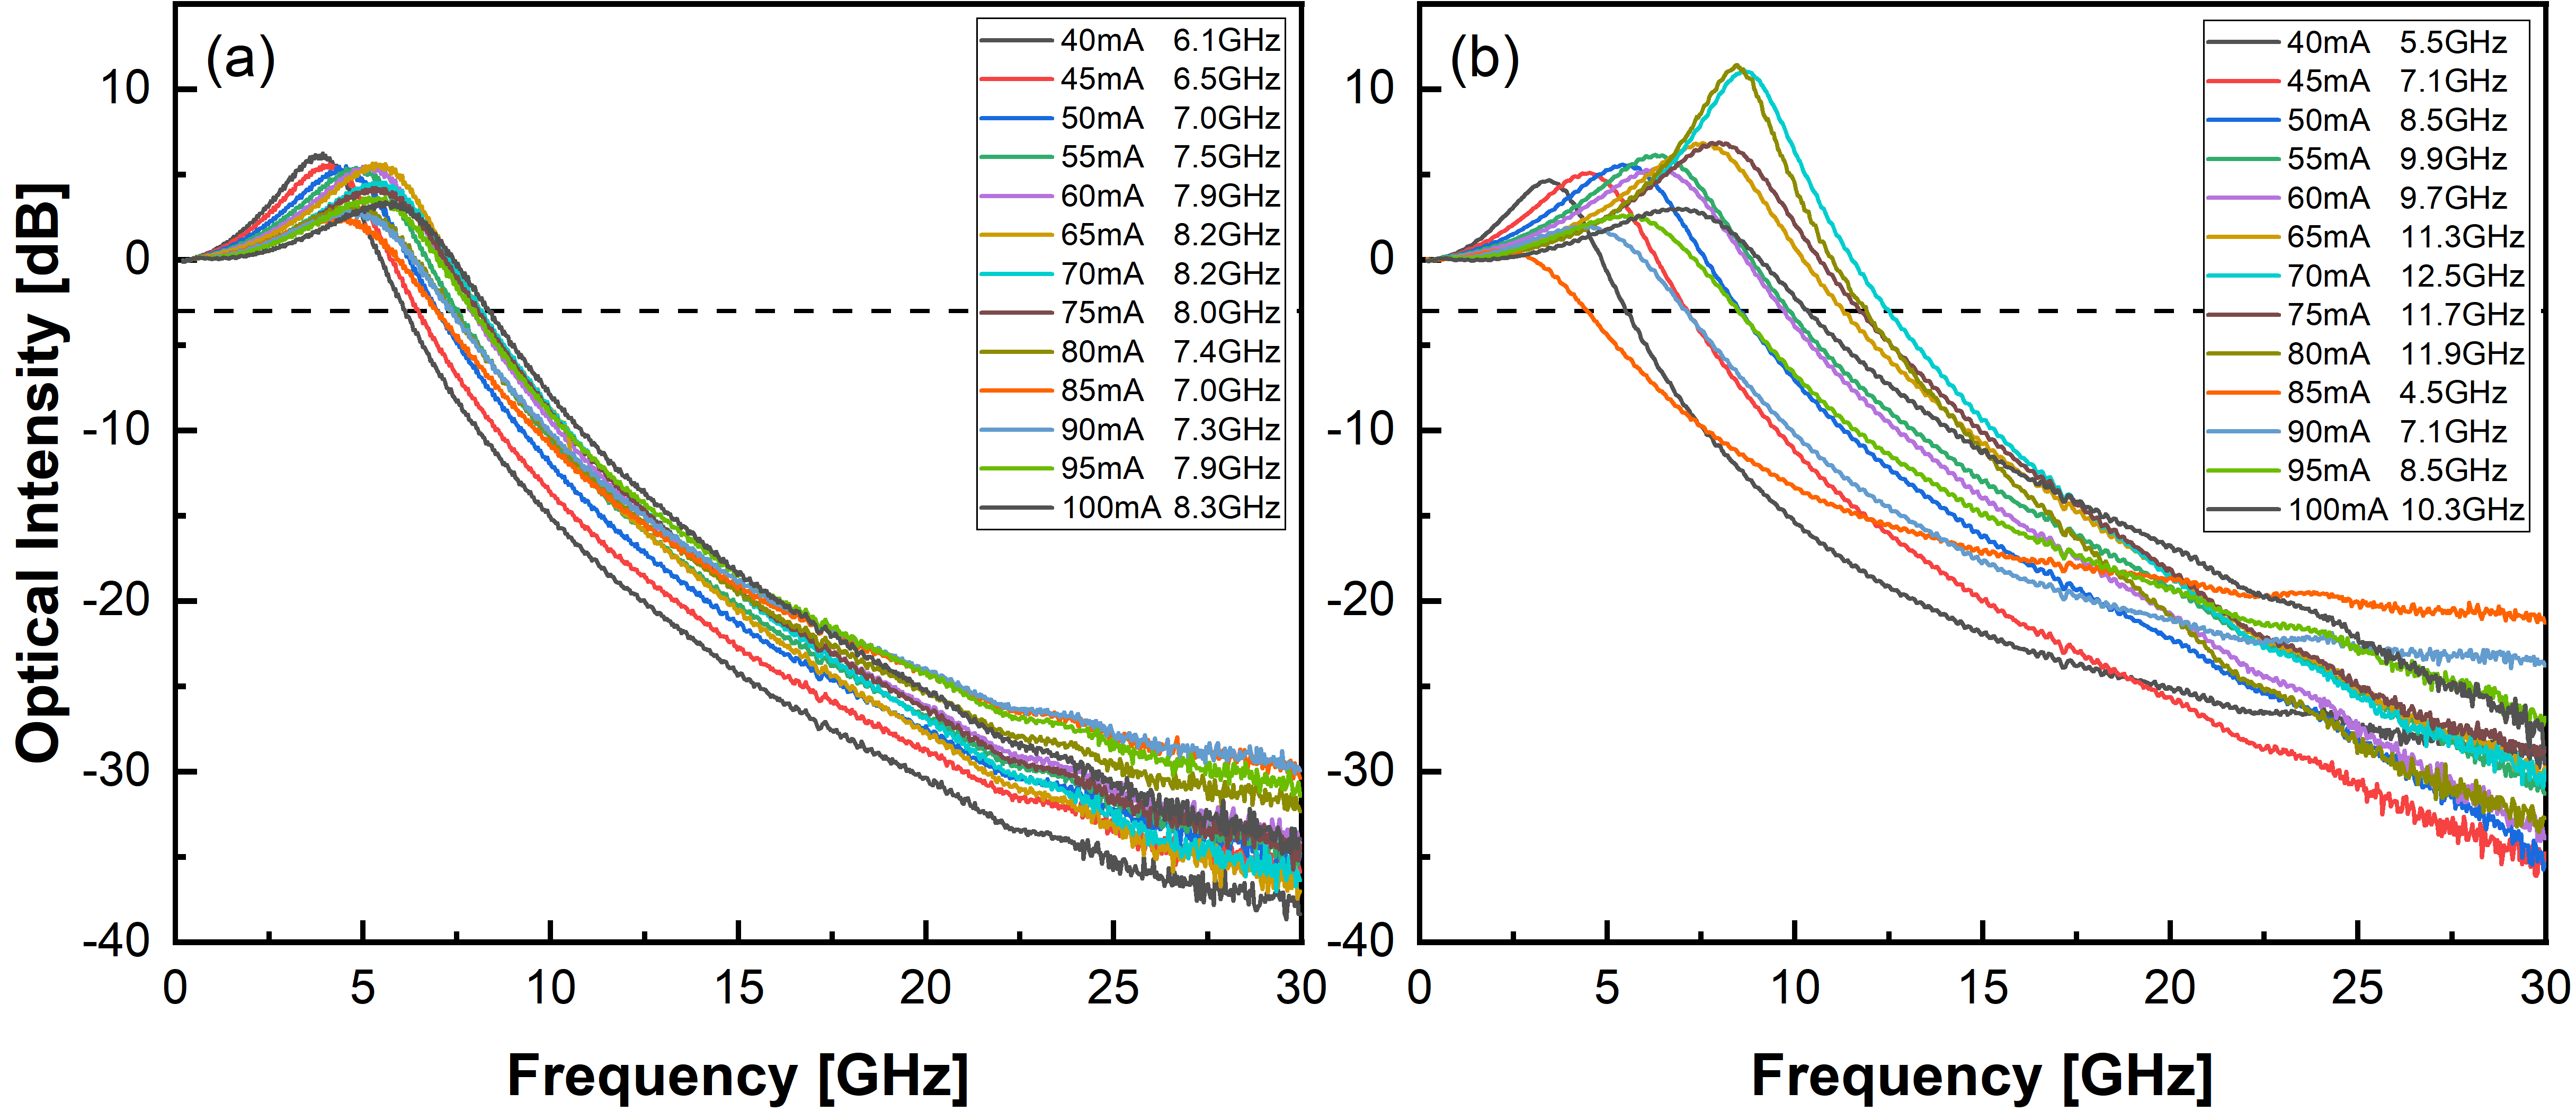
\includegraphics[width=\linewidth]{figures/bandwidth_gain_scan_cleaved_and_lensed_grating_4679.png}
    \caption{Bandwidth measurements of a normal tunable laser. (a) Without feedback, the $f_{3dB}$ show a normal behavior that first increase with the applied gain current and then decrease, (b) with feedback, the prominant peaks at 70 mA and 75 mA are due to the undamped RO peaks, at this condition, the $f_{3dB}$ got increased compare with the lase without feedback.}
    \label{fig:bandwidth_gain_scan_cleaved_and_lensed}
\end{figure}

% \begin{equation}
%     H(\omega)=\frac{\omega_R^2}{\omega_R^2-\omega^2-2j\omega\gamma}
%     \label{modulation_transfer_function}
% \end{equation}
% in \autoref{modulation_transfer_function}, $\omega_R$ is the relaxation resonance frequency and $\gamma$ is the damping factor.

% The relaxation oscillation frequency is a measure of the maximum modulation ability in semiconductor lasers through the injection current. Above the relaxation oscillation, the modulation efficiency is greatly degraded and intensity modulation through the injection current becomes difficult. [Semiconductor Lasers. Stability, Instability and Chaos.pdf]

\textit{The laser seeks a steady-state operation which maximizes feedback. When external feedback is present, the state corresponding to maximum feedback occurs when there is phase alignment  between the semiconductor cavity field and the reflected field. A carrier number change $n$ will change the resonance frequency of the semiconductor cavity. This in turn causes a phase change $\phi$ between the laser field and the reflected field. This acts to decrease the light intensity in proportion to $1-cos{\phi}\approx\frac{\phi^2}{2}$, which decreases the rate of stimulated emission and further increases $n$. This increase in $n$ again raises the cavity resonance frequency, causing the phase misalignment $\phi$ to continue to grow. Instability occurs for finite fluctuations of $\phi$ and $n$ when this effect becomes greater than the restoring forces giving rise to the relaxation oscillations described above.}

\textit{steady-state operation (phase alignment of the cavity field and reflected field)}

\textit{In steady-state operation, the laser with reflective feedback can be thought of as phase locked to the reflected field. The phenomenon that we describe is driven by large fluctuations in spontaneous emission that dislodge the laser from this locked state that is stable for small fluctuations. [Henry, Kazarinov 1986]}

\subsection{Detuend loading condition}\label{subsec:detuned_laoding_measurement}
Operating the tunable DBR laser under the detuned loading condition was measured and the result is shown in \autoref{fig:detuned_loading}. The measurement was performed by stabilizing the device at \SI{25}{\celsius} and using a gain current $I_{gain}$ of $75 \ mA$. When the laser is lasing on the slope of the grating response, the side modes have a different gain spectrum relative to the peak of the grating response, which introduces the asymmetric behavior of the side modes. In this case, when the left side mode is higher than the right one, means the lasing mode is operating at the longer wavelength side of the grating response, and vice versa. By increasing the phase current $I_{phase}$ from $14 \ mA$ to $20 \ mA$, the lasing mode is tuned from the longer wavelength side of the grating response to the shorter wavelength side. The maximum $f_{3dB}$ achieved at the longer wavelength side (red curve) is $10.6 \ GHz$ and the minimum (grey curve) is $8.5 \ GHz$. These two operating points also correspoinds to the red and grey points in \autoref{fig:PP_resonance_operation_principle}.

\begin{figure}[ht]
    \centering
    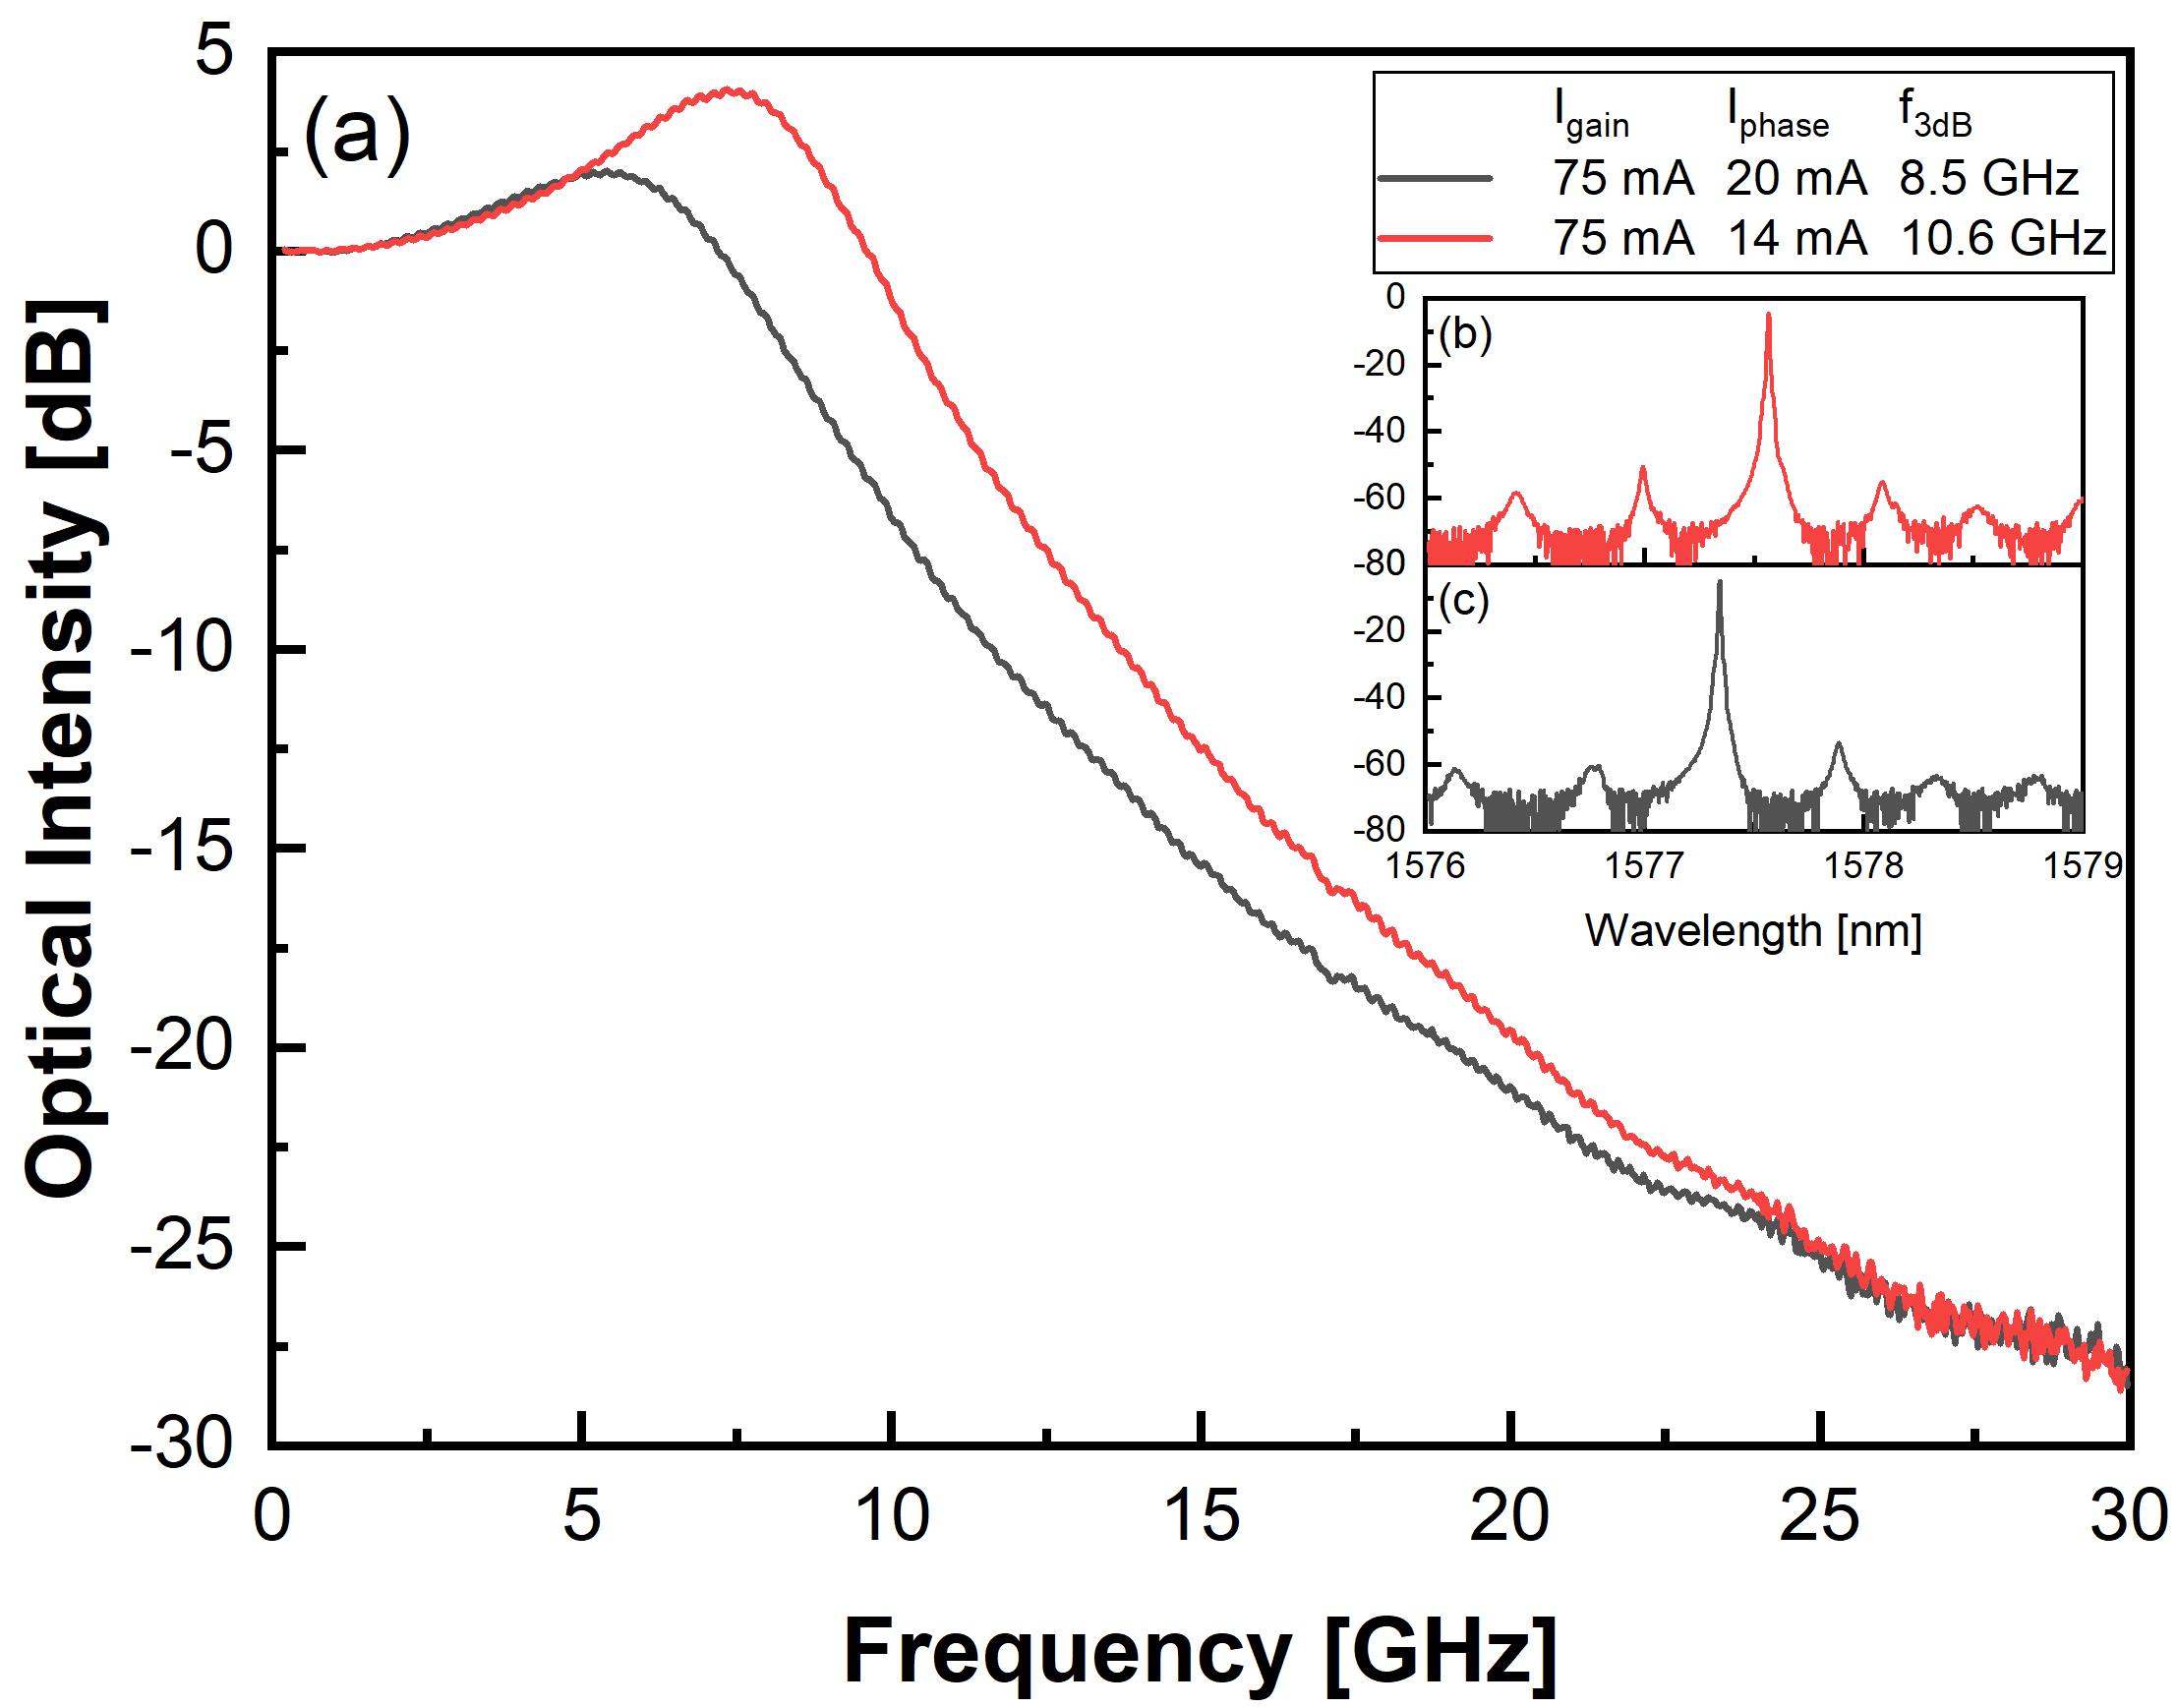
\includegraphics[width=.6\linewidth]{figures/detuned_loading.png}
    \caption{(a) Bandwidth enhancement with the detuned loading condition on DBR tunable laser. The red curve is detuned to the longer wavelength side of the grating response and it shows an increased bandwidth of 2.1 GHz compared to the grey curve without bandwidth enhancement effect. (b), (c) are the correspoinding spectra at these two operation points.}
    \label{fig:detuned_loading}
\end{figure}

\subsection{Undamped Relaxation Oscillation}\label{subsec:undamped_RO_measurement}
For the laser under undamped RO conditions, not all the undamped behavior lead to the good performance of the laser. As shown in \autoref{fig:undamped_RO}, the appearing of the undamped RO peak leads to the carrier-photon resonance appears at a higher relaxation oscillation frequency which permits a higher $f_{3dB}$ value. As the side peaks slowly move towards the main peak with increasing intensity, the carrier-photon resonance become stronger with a slightly decreased relaxation oscillating frequency. When more side peaks appear in \autoref{fig:undamped_RO} (c.1), the undamped RO behavior is very strong which lead to a broder lineshape and the intensity modulation shows prominent peaks with frequency correspoinding to the mode spacing of the side peaks. This last behavior leads to broadened lineshape and significantly decreases the $f_{3dB}$ compare to the other two cases.

\begin{figure}[ht]
    \centering
    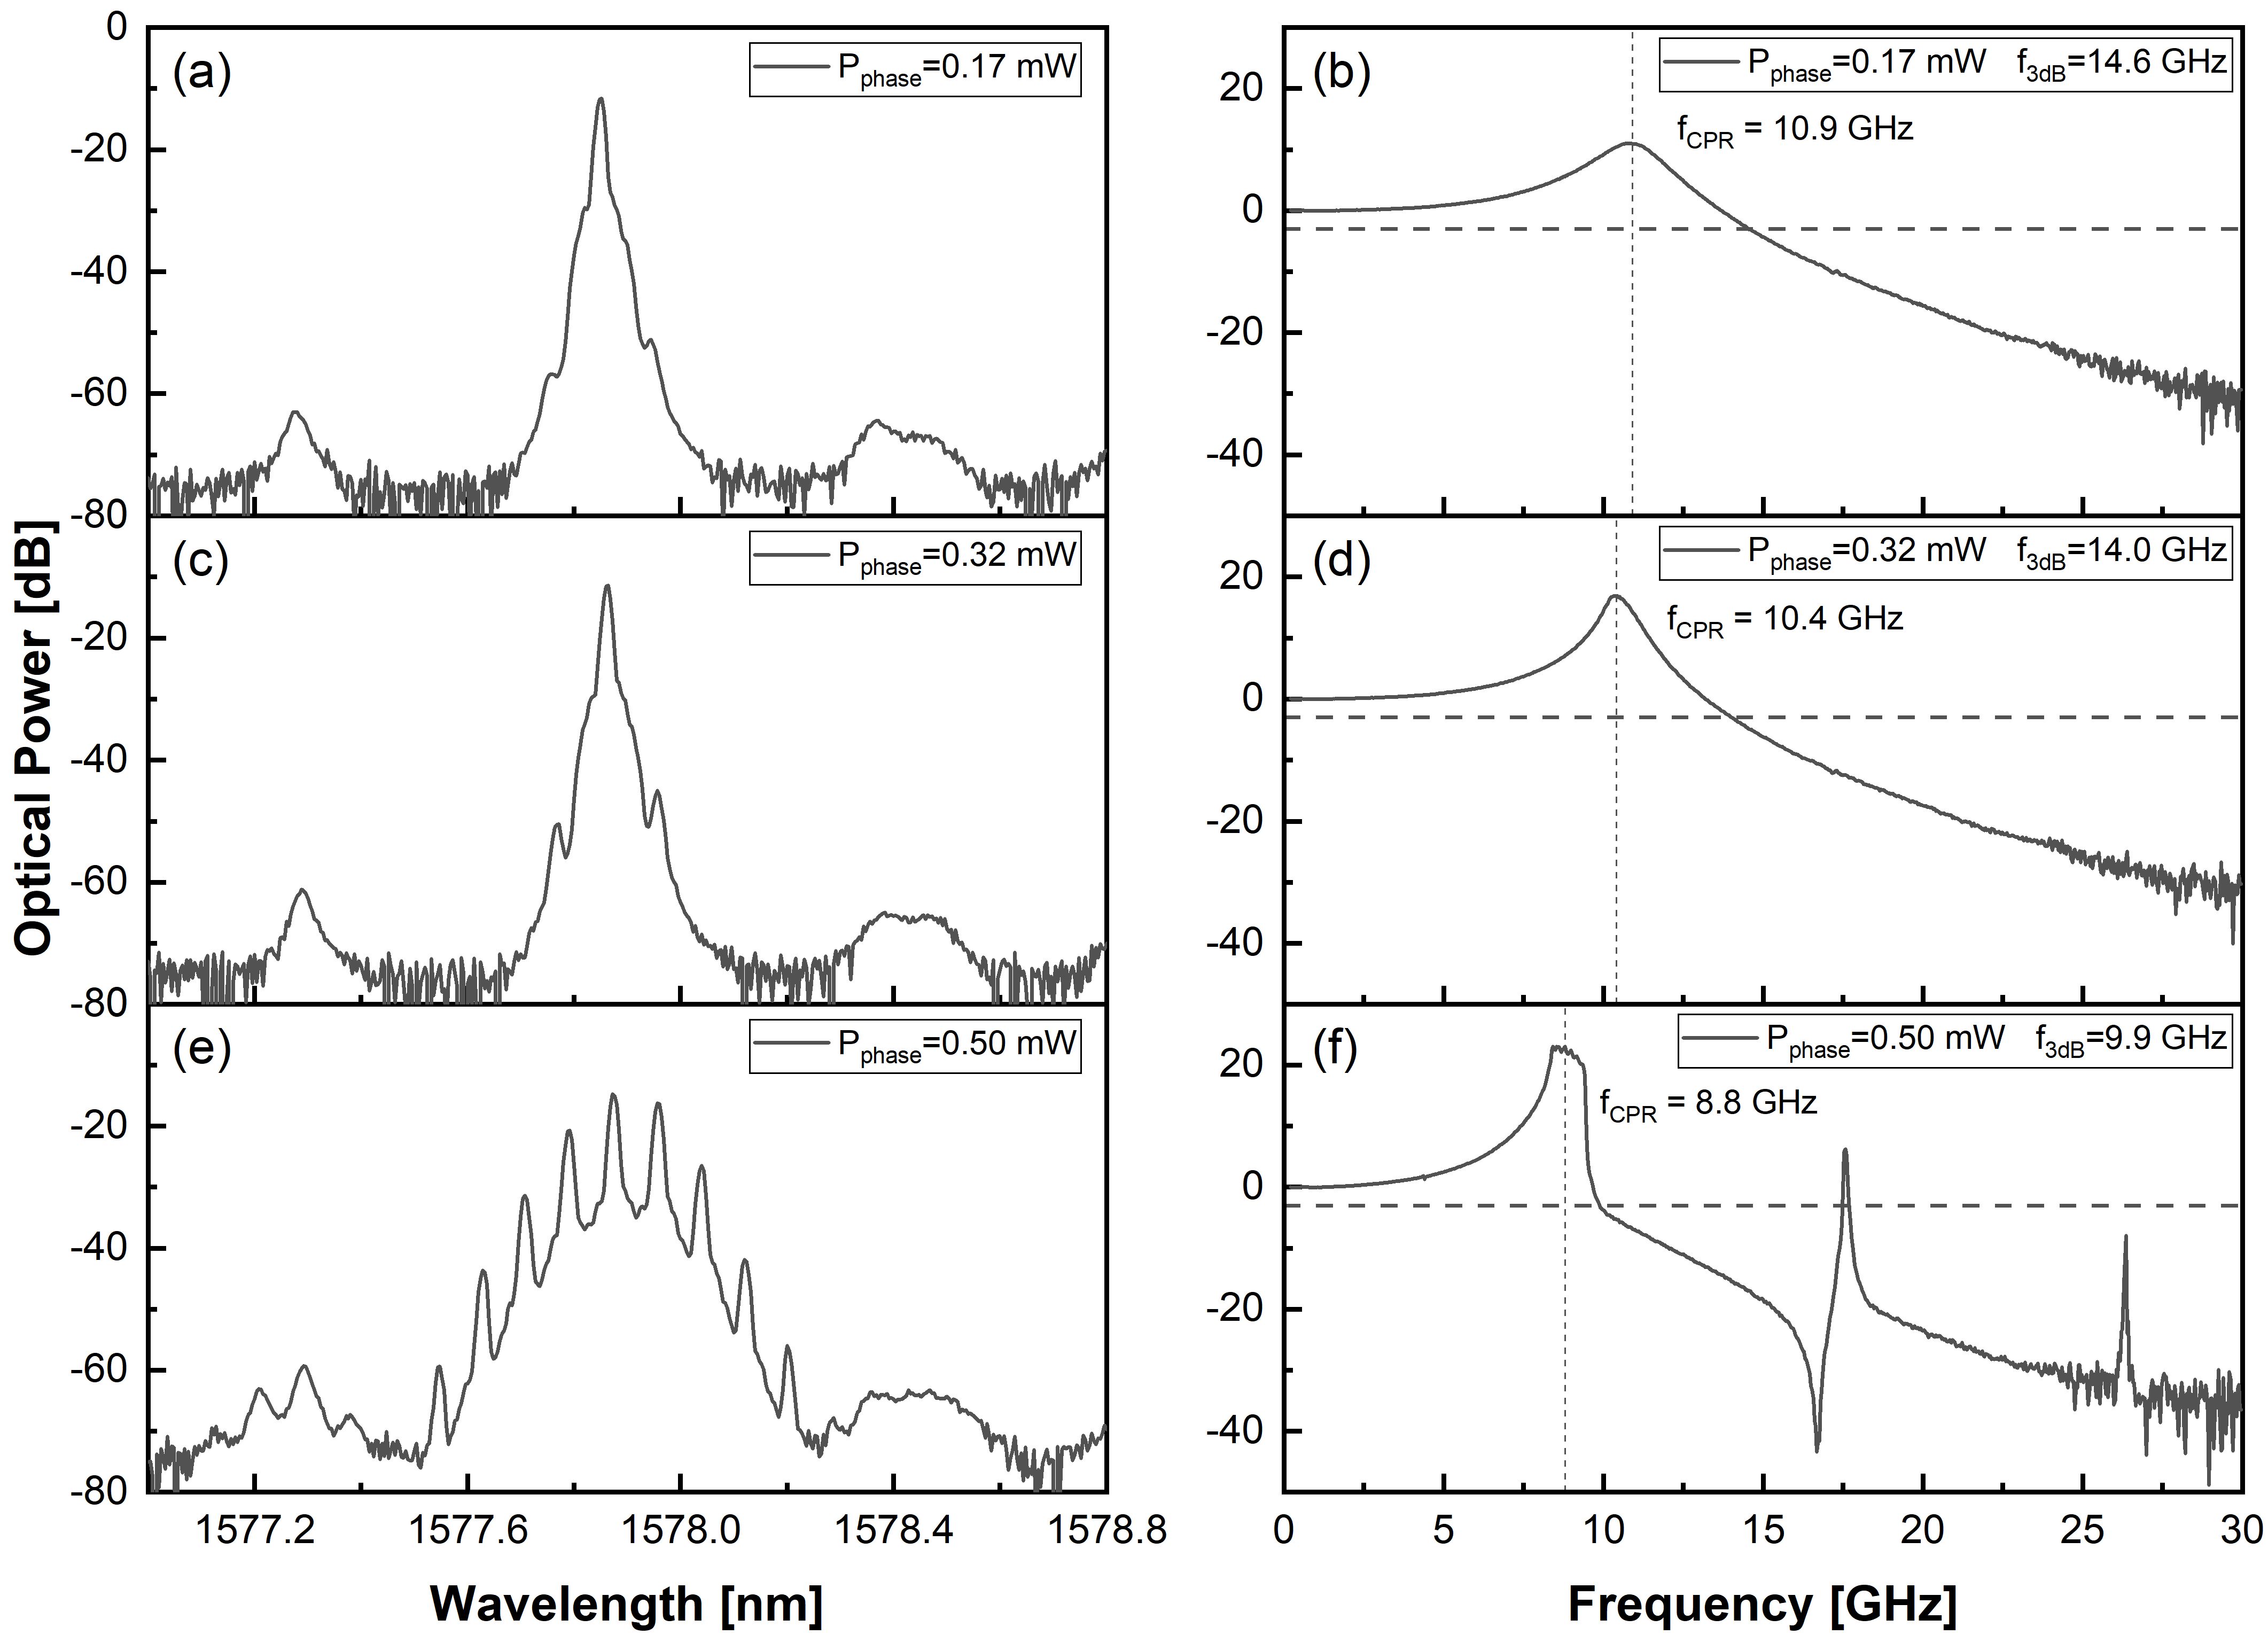
\includegraphics[width=\linewidth]{figures/Umdamped_RO_and_bandwidth_grating_4621.png}
    \caption{Laser spectra and their correspoinding intensity modulation curve. (a) Appearing of the undamped RO peak leads to a higher carrier-photon resonance in (b), (c) growing of the side peaks leads to increase of the carrier-photon resonance peak in (d), (e) drastic undamped RO leads to broadened lineshape and decreased modualiton bandwidth in (f).}
    \label{fig:undamped_RO}
\end{figure}

\subsection{}
\textit{Chirp arises because the frequency of the laser mode depends on the carrier number in the active region. Above threshold, the carrier number changes because of two effects: spectral hole burning prohibits the perfect pinning of the carrier number and permits adiabatic chirp, and during transients, there are relaxation oscillations of carrier number, which cause dynamic chirp. [Kazarinov 1987]}

\textit{Current modulation of the active region results in a modulation of both the photon density and the carrier density. The modulation of the carrier density modulates the gain; however, it also modulates the index of the active region na . As a result, the optical length of the cavity is modulated by the current, causing the resonant mode to shift back and forth in frequency. [Larry A. Coldren.pdf]}

If we consider the case discussed earlier where the semiconductor cavity is extended by a passive section of length $L_1$, with a nonreflective transition between the two sections, the reflection at the semiconductor section constant in magnitude, but has a frequency-dependent phase shift with $d\phi_r/d\omega = 2L_1/v_g1$ where $2L/v_g1$ is the roundtrip time in the external cavity. Therefore, in this case $B=0$, the chirp reduction factor is [Kazarinov 1987]



\section{Chirp Parameter Measurement}\label{sec:chirp_measurement}
($\alpha$-Factor)
Light chirping is a parasitic property of intensity modulated light. It originates in light emitters that produce a phase shift as the intensity is varied \cite{devaux1993simple}. Semiconductor lasers exhibit a particular nonlinearity in the interaction of the light with the active medium, which distinguishes them from all other lasers. The nonlinearity originates from the physics of the semiconductor band structure, since the photon generation typically occurs due to interband transitions. The gain spectrum of such lasers therefore does not exhibit a symmetric peak, as atomic transitions do, but has a strongly asymmetric shape. This affects the dispersive properties of the lasers as well, since those properties are connected via the Kramers-Kronig relation. As a consequence, the dispersion curve for the refractive index exhibits its zero crossing at higher frequency than the maximum of the gain spectrum. If the gain changes, e.g., by a change of the carrier density, the refractive index changes as well, which would not be the case for atomic transitions. Hence, changes in gain are in semiconductor lasers associated with changes in refractive index and vice versa. Since with a change of refractive index of the medium the optical frequency and thus the optical phase changes, one also speaks of amplitude phase coupling. A small change in the intensity (induced, e.g., by a change in the injection current, by dynamical instabilities, or even a spontaneous emission event) causes an excess perturbation of the phase of the lasing mode. In the rate equation description, the effect is taken into account via the so-called $\alpha$ parameter, which is also referred to as Henry parameter or linewidth enhancement factor. It is defined as
\begin{equation}
    \alpha=-\frac{\dv*{\chi_r(n)}{n}}{\dv*{\chi_i(n)}{n}}
\end{equation}

\subsection{Measurement with LCA}\label{subsec:measurement_with_LCA}
The network analyzer of \autoref{fig:LCA_setup} measures the small-signal frequency response of a light emitter, a dispersive medium and a light receiver. The dispersive medium is 81 $km$ of standard, single-mode fiber (zero dispersion at 1.3 $\mu m$) from and Er-doped fiber amplifiers pumped at 1.55 $\mu m$. Resonance frequencies are observed as sharp peaks in the frequency response.
\begin{figure}[ht]
    \centering
    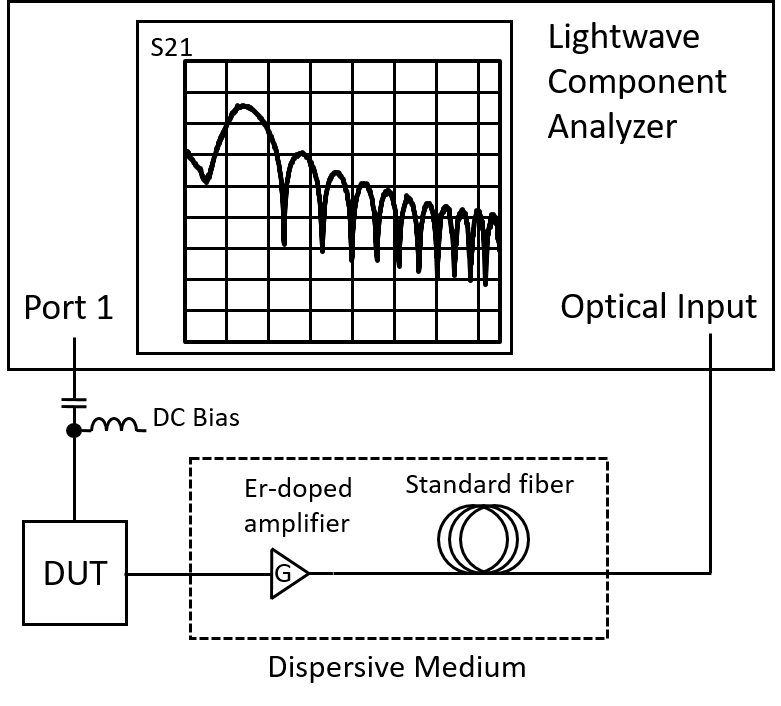
\includegraphics[width=.5\linewidth]{figures/LCA_setup.png}
    \caption{Schematic set-up for chirp parameter measurement.}
    \label{fig:LCA_setup}
\end{figure}

The resonance frequencies $f_u$ of Fig.2 corresponds to the $u^{th}$-zeros of xx. They follow a very simple law:
\begin{equation}
    f_u^2L=\frac{c}{2D\lambda ^2}(1+2u-\frac{2}{\pi}arctan(\alpha))
    \label{eq:LCA_equation}
\end{equation}

The equation is the result of two simultaneous interferences between the carrier and the two sidebands. Plotting $f_u^2L$ versus $2u$ gives a straight line whose slope and position yield the dispersion and the chirp parameter by liner regression.

\begin{figure}[ht]
    \centering
    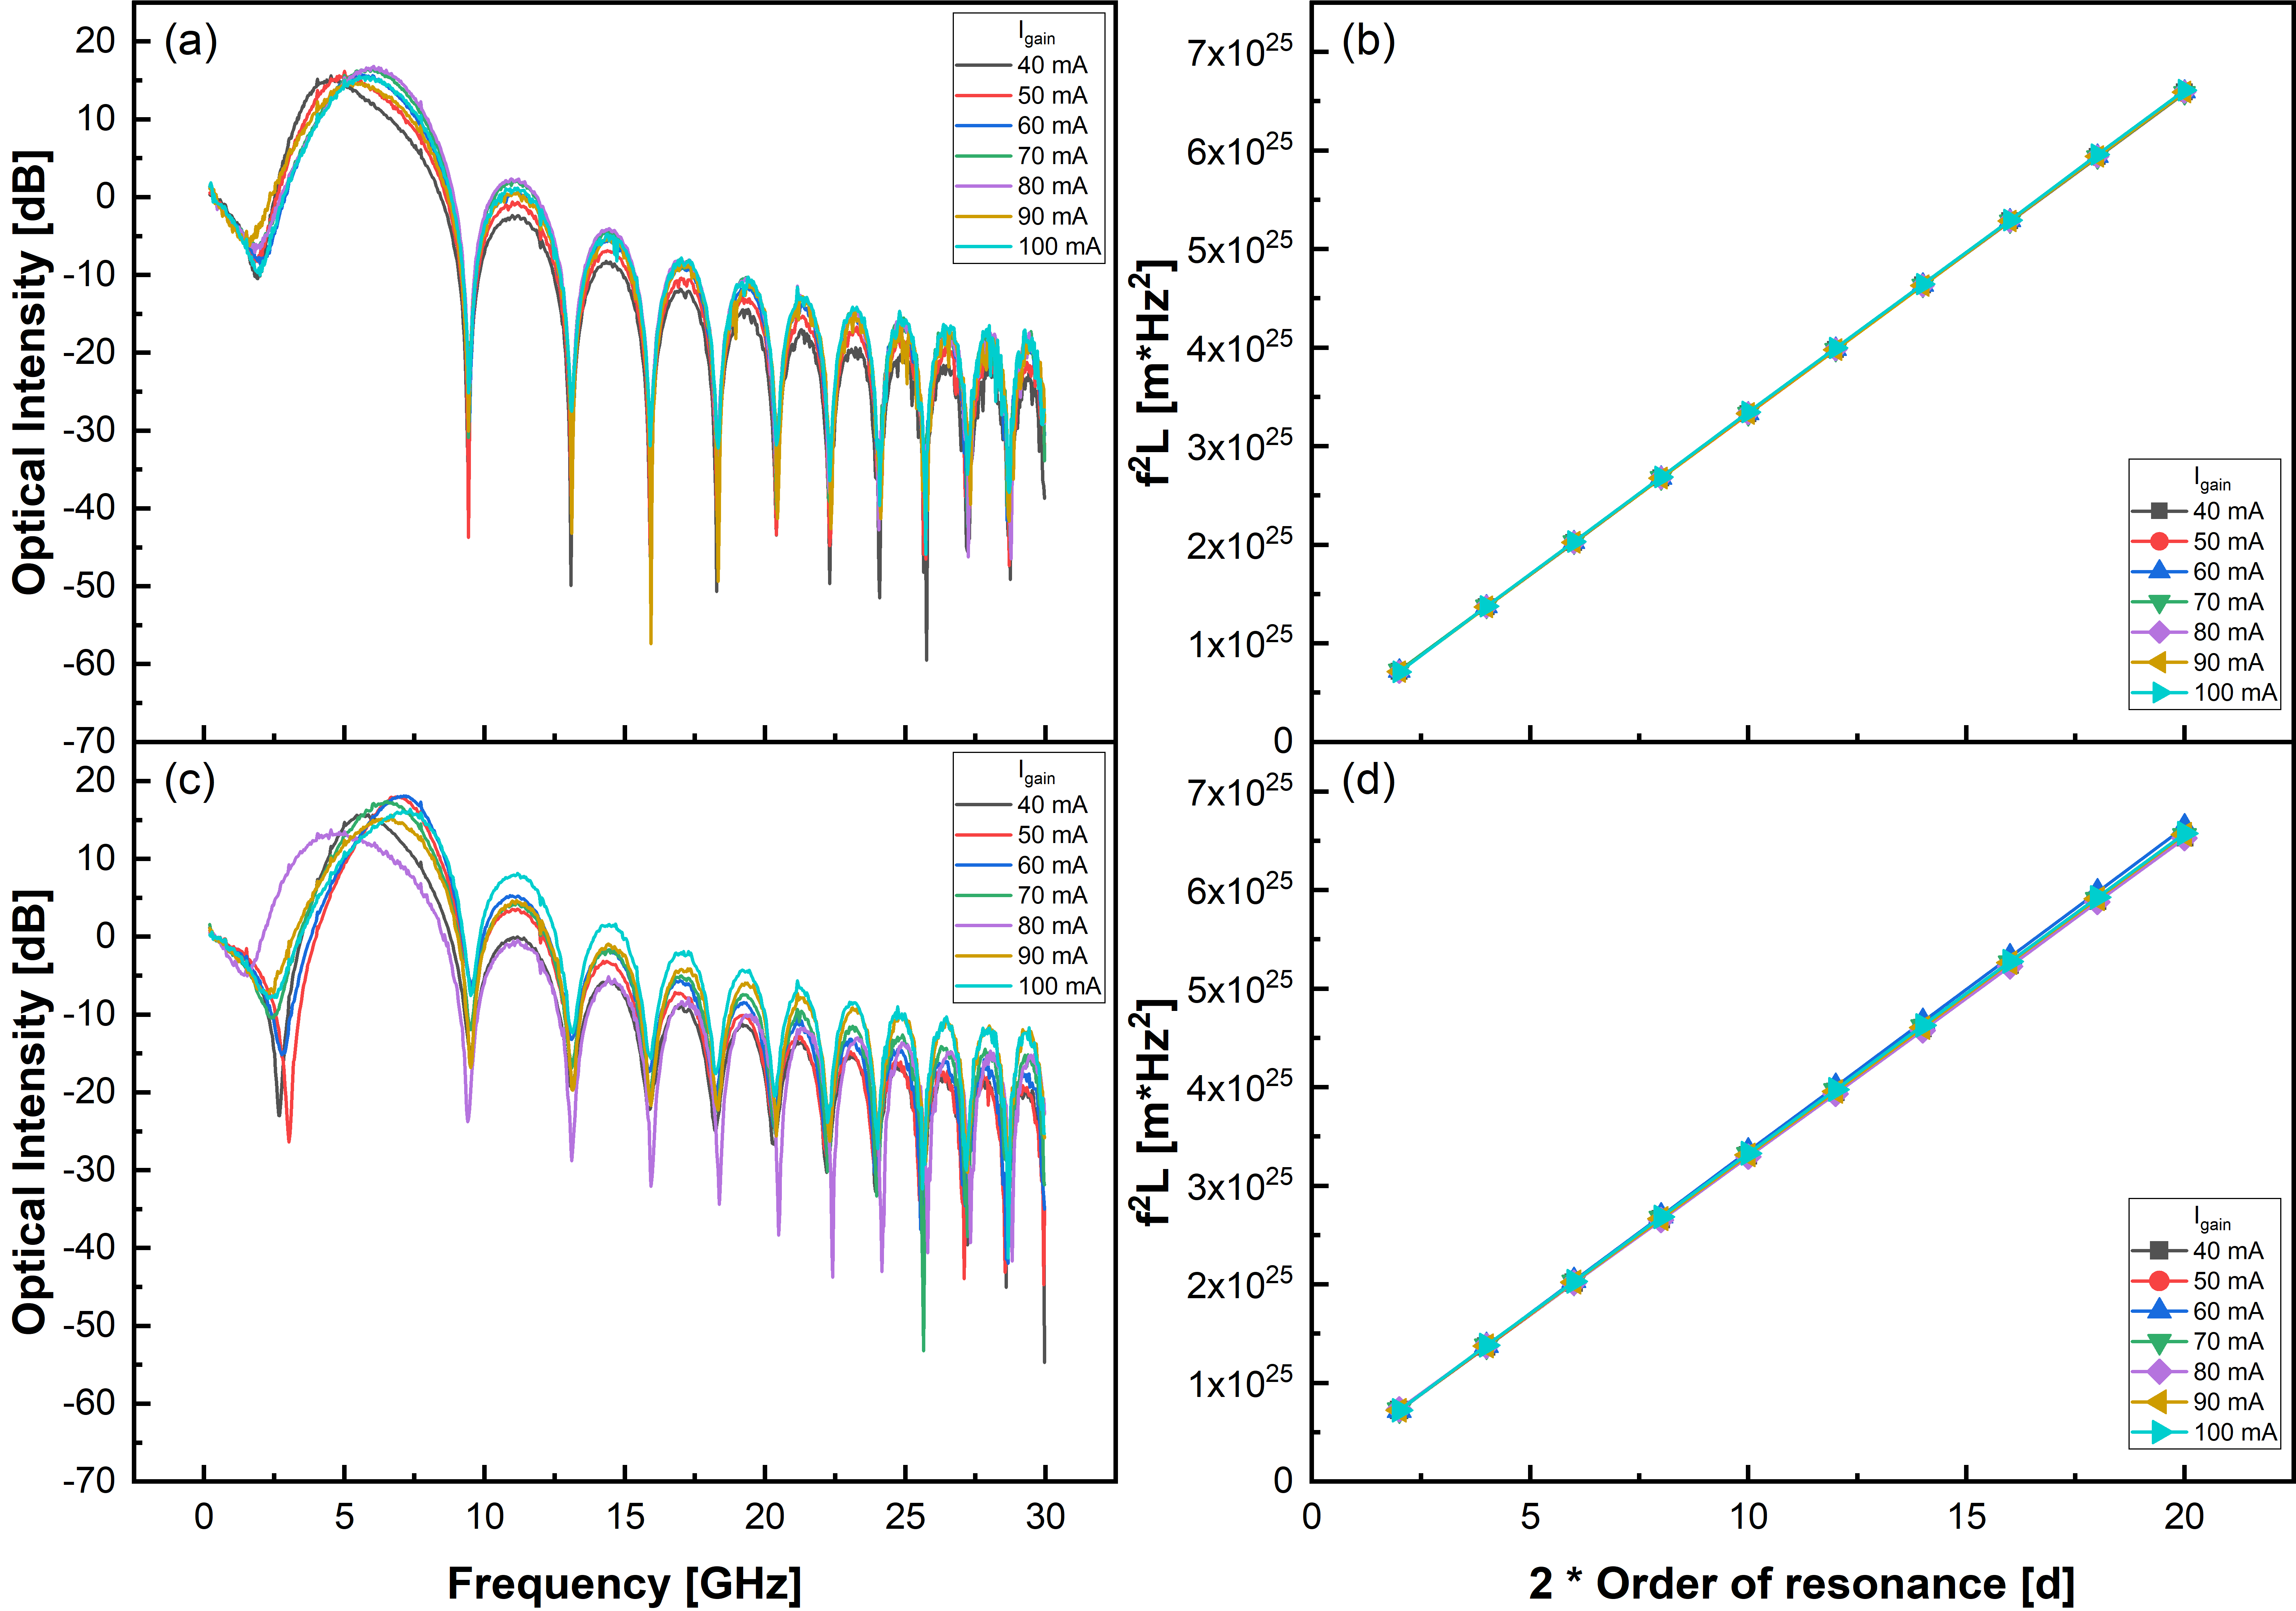
\includegraphics[width=\linewidth]{figures/chirp_cleaved_and_lensed_4679.png}
    \caption{}
    \label{fig:chirp_cleaved_and_lensed}
\end{figure}

% Please add the following required packages to your document preamble:
% \usepackage{booktabs}
% \usepackage{multirow}
\begin{table}[ht]
    \centering
    \caption{My caption}
    \label{my-label}
    \begin{tabular}{@{}lll@{}}
    \toprule
    \multirow{2}{*}{Current {[}mA{]}} & \multicolumn{2}{c}{$\alpha$} \\ \cmidrule(l){2-3} 
                                      & w/o feedback  & w/ feedback  \\ \midrule
    40                                & 3.164         & 2.499        \\
    50                                & 3.017         & 2.247        \\
    60                                & 2.687         & 2.439        \\
    70                                & 3.079         & 2.593        \\
    80                                & 3.003         & 3.095        \\
    90                                & 2.996         & 2.389        \\
    100                               & 2.605         & 2.472        \\ \bottomrule
    \end{tabular}
\end{table}

\subsection{AM-FM Index Method}
The experimental arrangement for measuring the intensity and phase modulation index is shown in Fig. 1. The semiconductor laser is biased above threshold and a small sinusoidally varying current at frequency $\Omega$ is superimposed. The intensity and spectral density of the radiation field are given by
\begin{equation}
    Intensity: E_0^2[1+mcos(\Omega t)]
\end{equation}
\begin{equation}
    Spectrum: Center \ line \ at \ \omega_1: E_0^2[J_0^2(\beta)+m^2J_1^2(\beta)]
    \label{eq:alpha_2}
\end{equation}
\begin{equation}
    First \ sidebands \ at \
    \ \omega_1 \pm \Omega: E_0^2\big\{J_1^2(\beta)+1[(m/2)(J_2(\beta)-J_0(\beta))]^2\big\}
    \label{eq:alpha_3}
\end{equation}

The phase modulation index $\beta$ can be found by measuring the relative sideband strength and using \autoref{eq:alpha_2} and \autoref{eq:alpha_3}. The factor $\alpha_m$ is then obtained as $\alpha_m = -2(\beta/m)$.
\begin{figure}[ht]
    \centering
    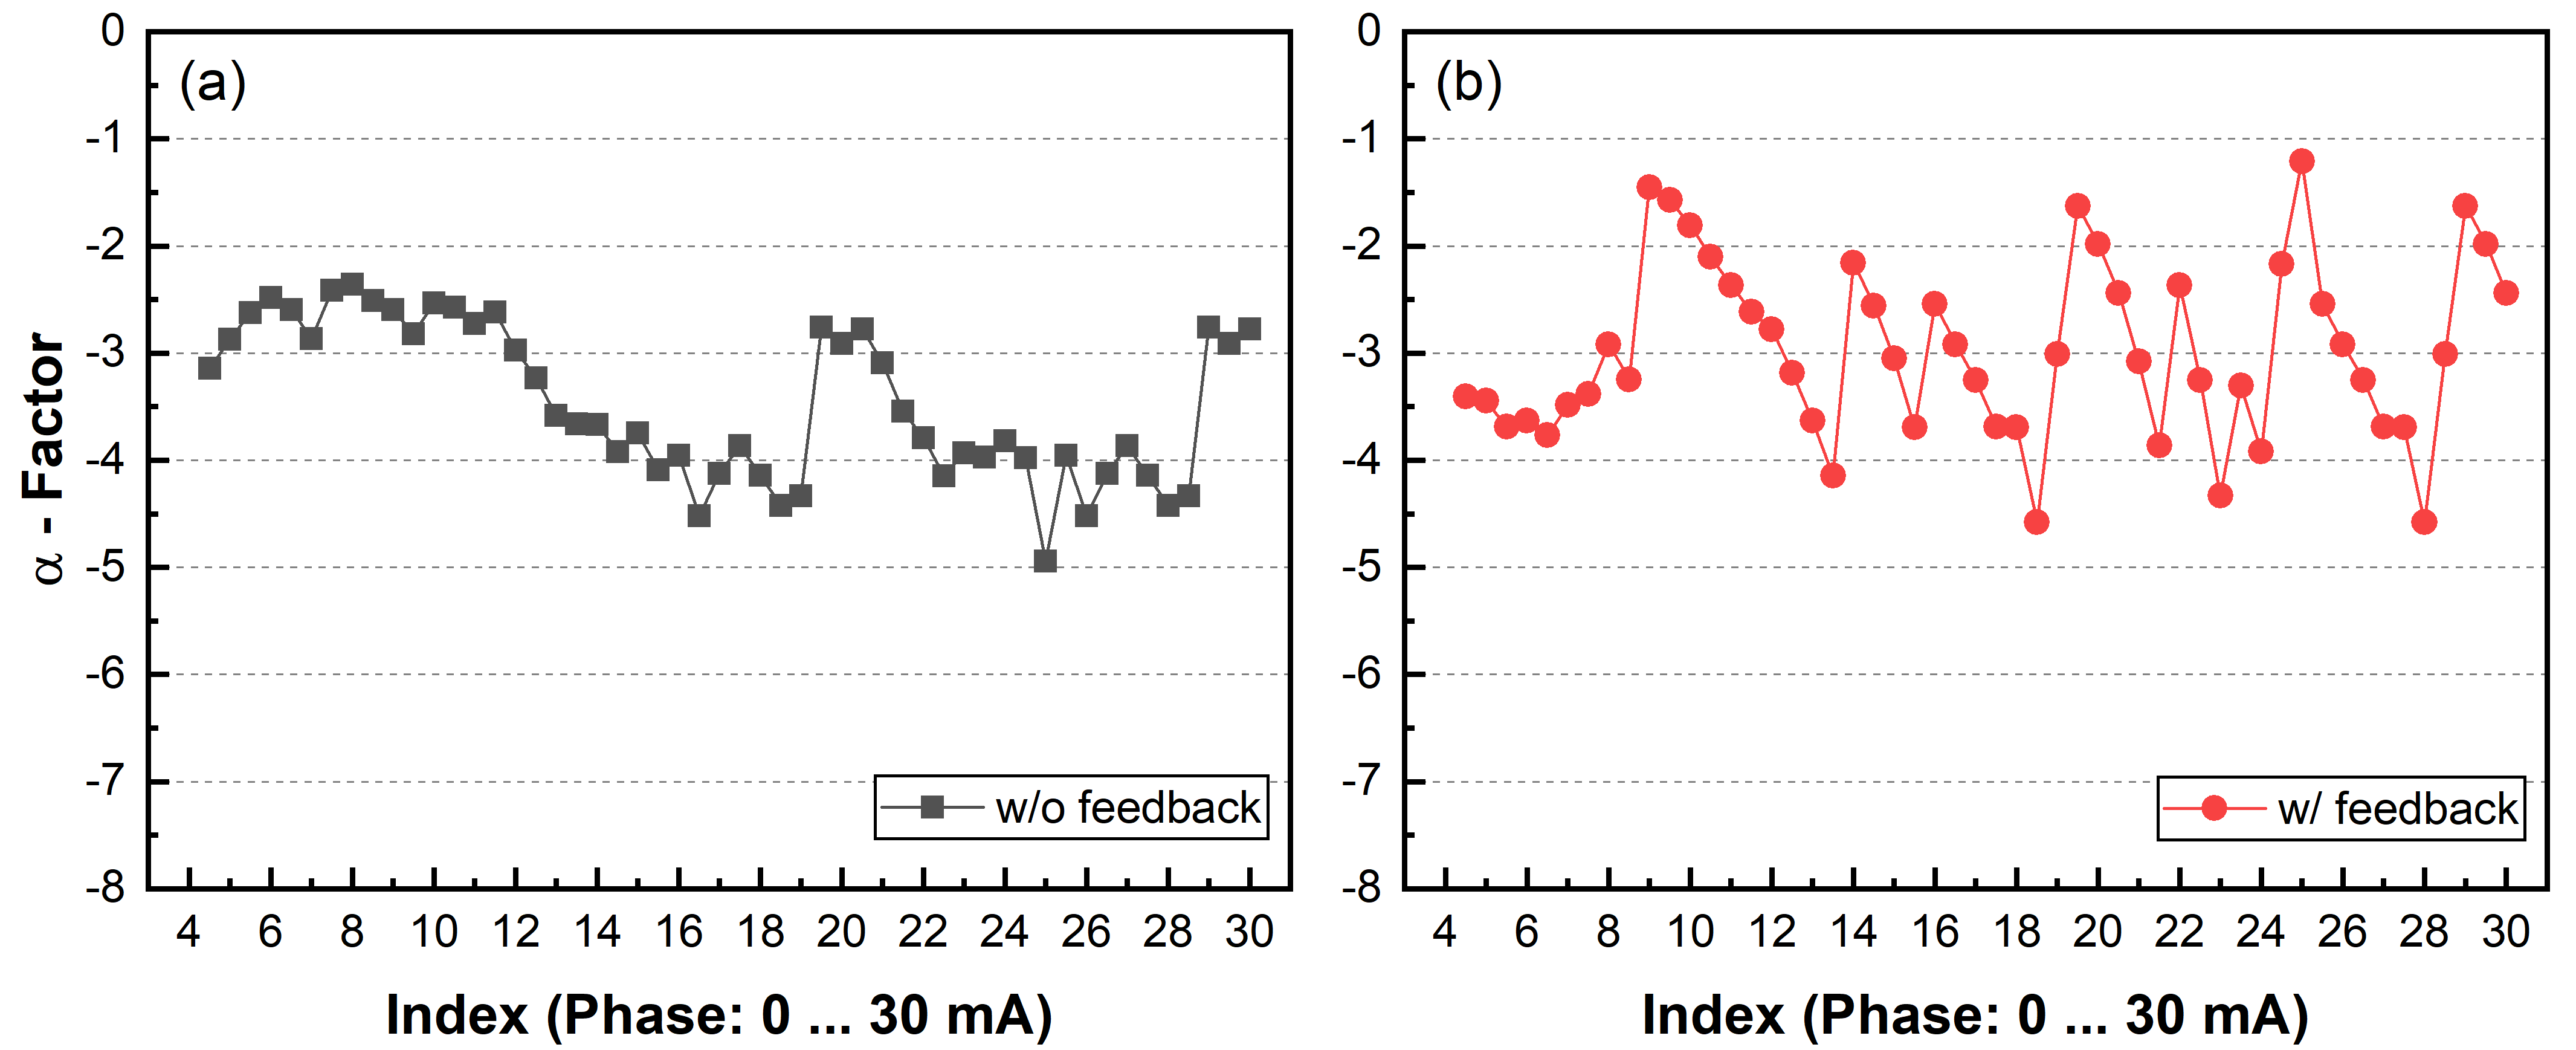
\includegraphics[width=\linewidth]{figures/Alpha_Cleaved_and_Lensed.png}
    \caption{Comparison of $\alpha$ parameter}
    \label{fig:Alpha_Cleaved_and_Lensed}
\end{figure}

\section{Phase Noise Measurement}

